\documentclass[11pt]{article}

\usepackage[utf8]{inputenc}
\usepackage[margin=1in]{geometry}
\usepackage{amsmath, amssymb, amsthm}
\usepackage{graphicx}
\usepackage{hyperref}
\usepackage{enumitem}
\usepackage{CJKutf8}
\usepackage{tikz}
\usetikzlibrary{arrows.meta, positioning}

\newtheorem{definition}{Definition}[section]
\newtheorem{theorem}{Theorem}[section]
\newtheorem{lemma}{Lemma}[section]
\newtheorem{remark}{Remark}[section]

\title{10-708 Probabilistic Graphical Models \\ Lecture Notes}
\author{}
\date{Spring 2026}

\begin{document}
\begin{CJK}{UTF8}{gbsn}
\maketitle
\tableofcontents
\newpage

% ============================================================
\section*{Math Foundations}
% ============================================================

\subsection*{概率基础}

\textbf{联合分布}：$p(x, y)$ = $x$ 和 $y$ 同时取某个值的概率。

\textbf{Marginal}：对不关心的变量求和掉。$p(x) = \sum_y p(x, y)$。

\textbf{Conditional}：固定一个变量的值。$p(x \mid y) = \frac{p(x, y)}{p(y)}$。

\textbf{Chain rule}：$p(x, y) = p(x) \cdot p(y \mid x) = p(y) \cdot p(x \mid y)$。

\textbf{Bayes rule}：从 chain rule 直接推出：$p(y \mid x) = \frac{p(x \mid y)\, p(y)}{p(x)}$。

\textbf{Independence}：$x \perp y$ 当且仅当 $p(x, y) = p(x)\, p(y)$。

\textbf{Conditional independence}：$x \perp y \mid z$ 当且仅当 $p(x, y \mid z) = p(x \mid z)\, p(y \mid z)$。

\subsection*{期望}

$\mathbb{E}_q[f(x)] = \sum_x q(x)\, f(x)$（离散），$= \int q(x)\, f(x)\, dx$（连续）。

物理写法：$\langle f(x) \rangle = \mathbb{E}[f(x)]$，尖括号 = 期望。

\subsection*{Log 和 Exp 的常用性质}

\begin{itemize}[nosep]
  \item $\log(ab) = \log a + \log b$（乘法变加法，这就是为什么 MLE 取 log）
  \item $\log \frac{a}{b} = \log a - \log b$
  \item $\log \exp(x) = x$，$\exp(\log x) = x$
  \item $\frac{d}{dx} \log x = \frac{1}{x}$，$\frac{d}{dx} e^x = e^x$
  \item $p \propto \exp(E)$ 意思是 $p = \frac{1}{Z}\exp(E)$（$\propto$ = 差一个归一化常数）
\end{itemize}

\subsection*{Entropy}

$H(q) = -\sum_x q(x) \log q(x) = -\mathbb{E}_q[\log q(x)]$。衡量分布的"不确定度"。

\begin{itemize}[nosep]
  \item $q$ 集中在一个点 $\to$ $H = 0$（完全确定）
  \item $q$ 是 uniform $\to$ $H$ 最大（最不确定）
  \item 独立分布的 entropy 可加：$H(q_1 q_2) = H(q_1) + H(q_2)$
\end{itemize}

\subsection*{KL Divergence}

$\mathrm{KL}(q \| p) = \sum_x q(x) \log \frac{q(x)}{p(x)} = \mathbb{E}_q[\log q - \log p] = -H(q) - \mathbb{E}_q[\log p]$。

\begin{itemize}[nosep]
  \item 衡量 $q$ 和 $p$ 之间的"距离"（但不对称：$\mathrm{KL}(q\|p) \neq \mathrm{KL}(p\|q)$）
  \item $\mathrm{KL}(q\|p) \geq 0$，等号当且仅当 $q = p$
  \item $\mathrm{KL}(q\|p)$：mode-seeking（$q$ 集中在 $p$ 的一个峰上）
  \item $\mathrm{KL}(p\|q)$：mode-covering（$q$ 覆盖 $p$ 的所有峰）
\end{itemize}

\subsection*{Lagrange Multiplier}

想 maximize $f(x)$ 但有约束 $g(x) = 0$。构造 $L = f(x) + \lambda \cdot g(x)$，对 $x$ 和 $\lambda$ 都求导令其为零。$\lambda$ 叫 Lagrange multiplier。

例子：maximize $H(q) = -\sum q_i \log q_i$ subject to $\sum q_i = 1$。

$L = -\sum q_i \log q_i + \lambda(\sum q_i - 1)$，对 $q_i$ 求导：$-\log q_i - 1 + \lambda = 0$，解出 $q_i = e^{\lambda - 1}$ = 常数 $\to$ uniform distribution。符合直觉：entropy 在 uniform 时最大。

\newpage

% ============================================================
\section*{Prerequisites: Key Concepts}
% ============================================================

\subsection*{What is inference?}

\textbf{Inference = asking questions about your model.} You have a model with known parameters, and you want to extract information from it. Any probabilistic question you ask counts as inference. For example:

\begin{itemize}[itemsep=4pt]
  \item $P(\text{disease} \mid \text{symptoms})$ --- given what you observed (symptoms), what's the probability of something you didn't observe (disease)? This is called a \textbf{conditional} query.
  \item $P(x_1)$ --- you don't care about the other variables, you just want the probability of $x_1$. This is called a \textbf{marginal} query (because you ``marginalize out'' everything else by summing over it: $P(x_1) = \sum_{x_2, x_3, \dots} P(x_1, x_2, x_3, \dots)$). Note: a conditional is really just two marginals divided: $P(A \mid B) = P(A, B) \,/\, P(B)$.
  \item $\arg\max_x P(x)$ --- what is the single most probable combination of all variables? This is called \textbf{MAP} (maximum a posteriori) inference.
  \item Draw random samples from $P(x)$ --- this is called \textbf{sampling}.
  \item Compute $Z$ --- the \textbf{partition function} (defined below).
\end{itemize}

These are all different \emph{types} of questions, but they are all inference because the model is fixed and you are extracting information from it.

The course highlights three types in particular because of their computational difficulty:
\begin{itemize}
  \item \textbf{Marginals and $Z$}: equally hard --- both are \emph{\#P-hard} (a class of counting problems even harder than NP).
  \item \textbf{MAP}: a different flavor of hard --- \emph{NP-hard} (an optimization problem, like solving a SAT instance).
\end{itemize}

\vspace{0.3em}
\noindent\fbox{\parbox{\dimexpr\textwidth-2\fboxsep-2\fboxrule}{%
\textbf{Inference vs.\ Learning.} \emph{Inference}: model is fixed, answer questions about it. \emph{Learning}: you don't know the model's parameters yet, and you want to find them from data. Learning is harder because each step of learning typically requires doing inference as a subroutine.
}}

\subsubsection*{MAP vs.\ MLE}

Both are ``$\arg\max$'' problems, but they optimize over different things:

\begin{center}
\begin{tabular}{l|cc}
  & \textbf{MAP} & \textbf{MLE} \\
  \hline
  What is fixed & model parameters $\theta$ & observed data \\
  What you optimize & variable assignment $\mathbf{x}$ & parameters $\theta$ \\
  Formula & $\arg\max_{\mathbf{x}}\, P(\mathbf{x})$ & $\arg\max_{\theta}\, P(\text{data} \mid \theta)$ \\
  Belongs to & Inference & Learning \\
\end{tabular}
\end{center}

\subsubsection*{Conditional vs.\ posterior}

Every \textbf{posterior} is a conditional, but not every conditional is called a posterior. The term \emph{posterior} specifically refers to the Bayesian update:
\[
  \underbrace{P(\theta \mid \text{data})}_{\text{posterior}}
  \;=\;
  \frac{
    \overbrace{P(\text{data} \mid \theta)}^{\text{likelihood}}
    \;\times\;
    \overbrace{P(\theta)}^{\text{prior}}
  }{
    \underbrace{P(\text{data})}_{\text{evidence (another }Z\text{!)}}
  }
\]
You start with a \textbf{prior} belief $P(\theta)$ about the parameters, observe data, then update to the \textbf{posterior} $P(\theta \mid \text{data})$ via Bayes' rule. In PGM literature, people often use ``conditional'' and ``posterior'' interchangeably for $P(z \mid x)$.

\subsection*{Bayesian reasoning}

Bayesian reasoning has three ingredients, chosen in this order:

\begin{enumerate}
  \item \textbf{Model family} (your choice of distribution type). For example: ``I'll model this data with a geometric distribution.'' This is fixed \emph{before} you see any data and is \emph{not} part of the prior.
  \item \textbf{Prior} $P(\theta)$ (your belief about the \emph{parameter values} before seeing data). For example: ``I think the success probability $p$ is somewhere between 0 and 1, I have no idea where, so I'll use a uniform prior on $[0,1]$.'' The prior is about $\theta$, not about which model to use.
  \item \textbf{Data} $x_1, x_2, \dots, x_n$ (what you observe).
\end{enumerate}

After observing data, Bayes' rule gives you the posterior:
\[
  P(\theta \mid \text{data})
  \;=\;
  \frac{P(\text{data} \mid \theta) \;\times\; P(\theta)}{P(\text{data})}
  \;\propto\;
  \underbrace{P(\text{data} \mid \theta)}_{\text{likelihood}} \;\times\; \underbrace{P(\theta)}_{\text{prior}}
\]

\subsubsection*{What if the prior is wrong?}

\textbf{A wrong prior is forgivable.} As you see more data, the likelihood dominates and the prior's influence fades. The posterior concentrates around the true parameter value regardless of where the prior started.

Example: you're flipping a coin that lands heads 90\% of the time. Your prior says $P(\text{heads}) = 0.5$. After 10 flips you might still be uncertain, but after 10{,}000 flips your posterior will be tightly concentrated near 0.9.

\subsubsection*{What if the model is wrong?}

\textbf{A wrong model is not forgivable.} If the true distribution is geometric but your model family only contains uniform distributions, no amount of data will recover the truth. The posterior will converge to whichever parameters make the uniform look ``as close as possible'' to the geometric---but it will never become geometric.

\vspace{0.3em}
\noindent\fbox{\parbox{\dimexpr\textwidth-2\fboxsep-2\fboxrule}{%
\textbf{Key distinction.} The \emph{prior} is your initial guess about parameter values---data corrects it. The \emph{model family} defines the space of distributions you can even consider---if the truth is not in that space, no amount of data helps.
}}

\subsection*{What is a partition function?}

A probability distribution has one hard rule: all probabilities must add up to 1.

In many models, we don't directly write down probabilities. Instead, we assign each outcome a \textbf{score} (an unnormalized number indicating how ``likely'' it is). For example:
\[
  \text{outcome } A: \text{score } 3, \qquad
  \text{outcome } B: \text{score } 5, \qquad
  \text{outcome } C: \text{score } 2.
\]
These scores add up to $3 + 5 + 2 = 10$, not 1. To turn them into valid probabilities, we divide each score by the total:
\[
  P(A) = \frac{3}{10}, \qquad P(B) = \frac{5}{10}, \qquad P(C) = \frac{2}{10}.
\]
That total---the number we divide by---is the \textbf{partition function} $Z$. In general:
\[
  \boxed{Z = \sum_{\text{all possible outcomes } x} f(x)}
  \qquad \text{so that} \qquad
  P(x) = \frac{f(x)}{Z}
\]
where $f(x)$ is the unnormalized score for outcome $x$.

\subsection*{Why is $Z$ a problem?}

With 3 outcomes, $Z$ is trivial. But in a graphical model with, say, 100 binary (0 or 1) variables, the number of possible outcomes is:
\[
  2^{100} \approx 10^{30}.
\]
Computing $Z$ means summing over \emph{all} $10^{30}$ scores. No computer can do this---the number of operations grows exponentially with the number of variables.

\subsection*{What is the likelihood function?}

Suppose you observe data $x_1, x_2, \dots, x_n$ and you have a model with parameters $\theta$. The \textbf{likelihood} asks: \emph{given these parameters $\theta$, how probable is the data I observed?}
\[
  L(\theta) \;=\; p(x_1 \mid \theta) \;\times\; p(x_2 \mid \theta) \;\times\; \cdots \;\times\; p(x_n \mid \theta)
\]
\textbf{Learning} = finding the $\theta$ that makes $L(\theta)$ as large as possible. This is called \textbf{maximum likelihood estimation (MLE)}.

\subsection*{Why does $Z$ block learning?}

Each $p(x_i \mid \theta)$ has $Z(\theta)$ hidden inside it:
\[
  p(x_i \mid \theta) = \frac{f_\theta(x_i)}{Z(\theta)},
  \qquad \text{where} \quad
  Z(\theta) = \sum_{\text{all } x} f_\theta(x).
\]
The numerator $f_\theta(x_i)$ is cheap---just plug in $x_i$. But the denominator $Z(\theta)$ requires summing over all possible outcomes. Worse: every time you try a new $\theta$ during optimization, $Z(\theta)$ changes, so you'd have to redo that impossible sum from scratch.

\vspace{0.5em}
\noindent\fbox{\parbox{\dimexpr\textwidth-2\fboxsep-2\fboxrule}{%
\textbf{Bottom line.} Almost everything we want to do---computing probabilities, marginals, learning parameters---requires $Z$, and $Z$ is intractable. The entire second half of this course is about methods that work \emph{around} this problem.
}}

% ============================================================
\section*{Big Picture: Post-Midterm Roadmap}
% ============================================================

With the $Z$ problem in mind, the course offers two categories of solutions:

\subsection*{Category 1: Inference (given a model, answer questions about it)}

\begin{itemize}
  \item \textbf{MCMC} (L9, L11): Generate samples from the distribution \emph{without} computing $Z$. (We will explain how later.)
  \item \textbf{Variational Inference} (L13): Instead of sampling, find a simpler distribution that is ``close'' to the true one, by solving an optimization problem. (We will define ``close'' precisely later.)
\end{itemize}

\subsection*{Category 2: Learning (train the model's parameters)}

\begin{enumerate}
  \item \textbf{EM} (L15): Uses variational inference as a building block to learn parameters of models with hidden variables.
  \item \textbf{VAE} (L16): Scales EM to work with neural networks.
  \item \textbf{GAN} (L17--18): Gives up on likelihood entirely. Uses an adversarial game between two networks instead.
  \item \textbf{Score Matching} (L19): Also gives up on $Z$. Instead of matching the distribution itself, matches its \emph{gradient}---and $Z$ conveniently disappears when you take the gradient. (We will show why later.)
\end{enumerate}

\subsection*{Dependency structure}

\begin{center}
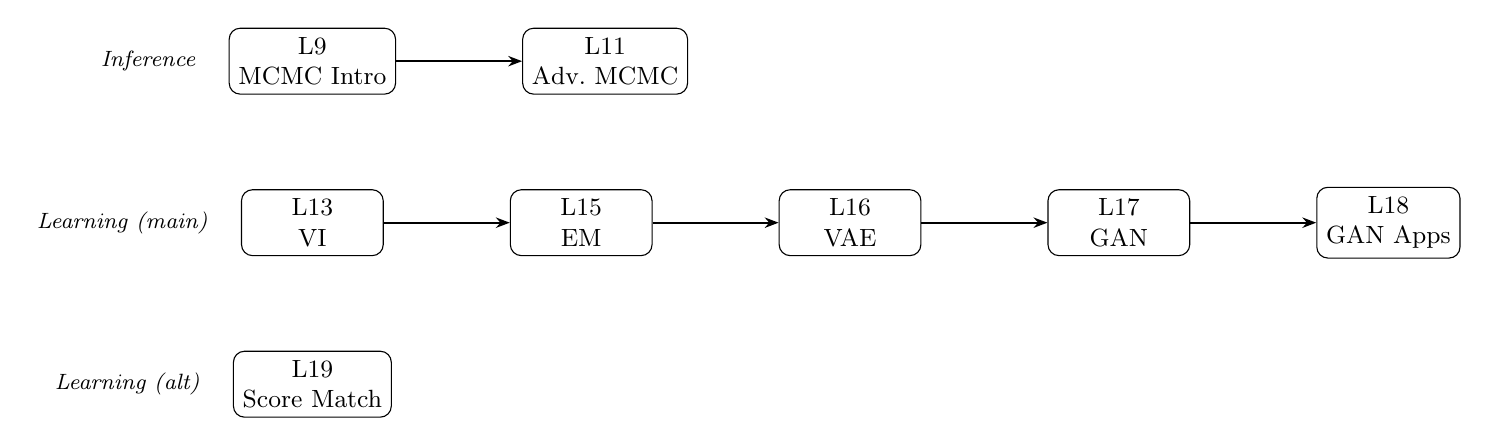
\begin{tikzpicture}[
    node distance=0.4cm and 1.6cm,
    every node/.style={font=\small},
    box/.style={draw, rounded corners, minimum height=0.8cm, minimum width=1.8cm, align=center},
    arr/.style={-{Stealth[length=5pt]}, thick}
  ]
  % MCMC track
  \node[box] (l9)  {L9\\MCMC Intro};
  \node[box, right=of l9] (l11) {L11\\Adv.\ MCMC};
  \draw[arr] (l9) -- (l11);

  % VI track
  \node[box, below=1.2cm of l9] (l13) {L13\\VI};
  \node[box, right=of l13] (l15) {L15\\EM};
  \node[box, right=of l15] (l16) {L16\\VAE};
  \node[box, right=of l16] (l17) {L17\\GAN};
  \node[box, right=of l17] (l18) {L18\\GAN Apps};
  \draw[arr] (l13) -- (l15);
  \draw[arr] (l15) -- (l16);
  \draw[arr] (l16) -- (l17);
  \draw[arr] (l17) -- (l18);

  % Score matching
  \node[box, below=1.2cm of l13] (l19) {L19\\Score Match};

  % Labels
  \node[left=0.3cm of l9, anchor=east, font=\footnotesize\itshape] {Inference};
  \node[left=0.3cm of l13, anchor=east, font=\footnotesize\itshape] {Learning (main)};
  \node[left=0.3cm of l19, anchor=east, font=\footnotesize\itshape] {Learning (alt)};
\end{tikzpicture}
\end{center}

\newpage

% ============================================================
\section{Introduction}
% Lecture 1
% ============================================================


% ============================================================
\section{Directed Graphical Models (Bayesian Networks)}
% Lecture 2
% ============================================================


% ============================================================
\section{Undirected Graphical Models (MRFs)}
% Lectures 3--4
% ============================================================


% ============================================================
\section{Exact Inference}
% Lecture 5
% ============================================================


% ============================================================
\section{Belief Propagation}
% Lectures 6--7
% ============================================================


% ============================================================
\section{Graph Neural Networks}
% Lecture 8
% ============================================================


% ============================================================
\section{MCMC Introduction}
% Lecture 9
% ============================================================

\subsection{背景：为啥需要 MCMC}

\textbf{问题}：你有个分布 $p(x) \propto \exp(-E(x))$，知道 $E(x)$（unnormalized），但
\begin{itemize}[nosep]
  \item 不知道 $Z = \int \exp(-E(x)) dx$（高维 intractable）
  \item 没法直接采样（不像 Gaussian 有 inverse CDF）
  \item 想算 $\mathbb{E}_p[f(x)]$
\end{itemize}

\textbf{Monte Carlo}：用 sample average 近似 expectation $\mathbb{E}_p[f(x)] \approx \frac{1}{N} \sum_i f(x_i)$，$x_i \sim p$。但前提是你得能采样。

\textbf{MCMC 的 trick}：构造一条 \textbf{Markov chain} $x_0 \to x_1 \to x_2 \to \cdots$，使得它的 \textbf{stationary distribution} 等于 $p$。跑足够久，链上的状态就近似从 $p$ 采的。

\subsection{核心定义}

\begin{definition}[Markov chain]
$x_{t+1}$ 的分布只依赖于 $x_t$，不依赖更早的历史：
\[
P(x_{t+1} | x_t, x_{t-1}, \ldots) = P(x_{t+1} | x_t)
\]
Transition 完全由 $P(x \to x')$ 决定。
\end{definition}

\begin{definition}[Stationary distribution]
分布 $\pi$ 是 Markov chain 的 stationary distribution 如果
\[
\pi(x') = \sum_x \pi(x) P(x \to x')
\]
意思是：如果当前状态分布是 $\pi$，下一步还是 $\pi$（不动点）。在合理条件下（irreducible + aperiodic），任何初始分布都会收敛到 $\pi$。
\end{definition}

\begin{definition}[Detailed balance]
Markov chain 对分布 $\pi$ 满足 detailed balance 如果
\[
\pi(x) P(x \to x') = \pi(x') P(x' \to x) \quad \forall x, x'
\]
意思是 $x$ 和 $x'$ 之间双向"概率流"相等。
\end{definition}

\begin{lemma}
Detailed balance $\Rightarrow$ stationarity。即如果 $\pi$ 满足 detailed balance，那 $\pi$ 是 stationary distribution。
\end{lemma}

\textbf{证明}（一行）：
\[
\sum_x \pi(x) P(x \to x') = \sum_x \pi(x') P(x' \to x) = \pi(x') \sum_x P(x' \to x) = \pi(x')
\]
（用 detailed balance 把 $\pi(x) P(x \to x')$ 换成 $\pi(x') P(x' \to x)$，然后 $\sum_x P(x' \to x) = 1$。）

\textbf{反过来不成立}：stationary 不一定 detailed balance。Detailed balance 是更强的条件（implies time-reversibility）。但实际中设计 MCMC 算法时，一般通过 detailed balance 来\textbf{保证} stationarity——比验证一般 stationarity 容易。

\subsection{Metropolis-Hastings (MH)}

最 general 的 MCMC 算法。

\textbf{Setup}：要采的目标分布 $\pi(x) \propto \exp(-E(x))$。选一个 proposal distribution $q(x' | x)$（通常是 symmetric，比如 $x' = x + $ Gaussian noise）。

\textbf{算法}：
\begin{enumerate}[nosep]
  \item 当前状态 $x$，从 $q(x' | x)$ proposes 一个 $x'$
  \item 计算 acceptance ratio
  \[
  \alpha(x \to x') = \min\!\left(1, \frac{\pi(x') q(x | x')}{\pi(x) q(x' | x)}\right)
  \]
  \item 以概率 $\alpha$ 接受 $x'$；否则留在 $x$
\end{enumerate}

\textbf{为啥这样设计}：可以验证这个 transition 满足 detailed balance for $\pi$（由 $\alpha$ 的形式直接保证）。

\textbf{$Z$ 自动消}：注意 acceptance ratio 是 $\pi(x') / \pi(x) = \exp(E(x) - E(x'))$，$Z$ 在分子分母 cancel。\textbf{所以 MH 不需要 $Z$ 也能采样}。这是 MCMC 的核心卖点。

\textbf{Symmetric proposal} ($q(x'|x) = q(x|x')$) 时，$\alpha = \min(1, \pi(x')/\pi(x))$ 简化为：
\begin{itemize}[nosep]
  \item $\pi(x') > \pi(x)$（"上坡"）：肯定接受
  \item $\pi(x') < \pi(x)$（"下坡"）：以概率 $\pi(x')/\pi(x)$ 接受
\end{itemize}
直觉：链 prefers 高概率区域，但偶尔接受低概率提议（保证 detailed balance）。

\subsection{Gibbs Sampling}

\textbf{高维专用}。当 $x = (x_1, \ldots, x_d)$ 是高维向量时，从 joint $p(x)$ 提议很难，但从 conditional $p(x_i | x_{-i})$ 通常容易。

\textbf{算法}（systematic scan）：
\begin{enumerate}[nosep]
  \item 当前 $x = (x_1, \ldots, x_d)$
  \item 从 $p(x_1 | x_2, x_3, \ldots, x_d)$ 采新 $x_1$
  \item 从 $p(x_2 | x_1^{\text{new}}, x_3, \ldots, x_d)$ 采新 $x_2$
  \item $\ldots$
  \item 从 $p(x_d | x_1^{\text{new}}, \ldots, x_{d-1}^{\text{new}})$ 采新 $x_d$
  \item Repeat
\end{enumerate}
（也有 random scan 版本，每次随机选一个 coordinate 更新。）

\textbf{为啥 conditional 容易}：在 PGM 里，$p(x_i | x_{-i}) = p(x_i | \text{Markov blanket of } x_i)$。Markov blanket 通常很小，conditional 是个低维分布。

\textbf{Gibbs 是 MH 的特例}：Gibbs 等价于 MH with proposal $q(x'|x) = p(x'_i | x_{-i})$，acceptance ratio = 1（永远接受）。

\textbf{Stationarity}：每个 conditional update 都 preserves $p$（因为 $p(x_i | x_{-i})$ 是从正确分布采）。Cycle 一遍所有 coordinate 之后还是 $p$。

\subsection{Langevin Dynamics（连续空间）}

\paragraph{物理出处}

法国物理学家 Paul Langevin 1908 年研究 Brownian motion 时写的方程。原始 setup：\textbf{在 potential $E(x)$ 里运动的粒子，受到摩擦 + 随机热噪声}：
\[
\dot{x} = -\nabla E(x) + \text{thermal noise}
\]
平衡态下粒子的位置分布是 Boltzmann 分布 $\propto \exp(-E / k_B T)$。

ML 把这个借过来：把 "平衡态分布" 当成你想采样的目标，\textbf{让粒子跑 Langevin dynamics，跑久了它的位置就近似从目标分布采的}。

\paragraph{离散化的更新规则}

\[
\boxed{x_{t+1} = x_t - \eta \nabla_x E(x_t) + \sqrt{2 \eta} \, \xi_t, \quad \xi_t \sim \mathcal{N}(0, I)}
\]
两部分：
\begin{itemize}[nosep]
  \item $-\eta \nabla_x E(x_t)$: \textbf{gradient descent on energy}（往 $E$ 低的方向走 = 往 $p$ 高的方向走）
  \item $\sqrt{2\eta}\, \xi_t$: \textbf{Gaussian noise}（每步加一点随机扰动）
\end{itemize}

连续 SDE 形式（$\eta \to 0$ 极限）：
\[
dx_t = -\nabla_x E(x_t) dt + \sqrt{2} \, dW_t
\]

\paragraph{直觉：exploit + explore}

\begin{itemize}[nosep]
  \item \textbf{没有 noise} $\to$ 纯 gradient descent $\to$ 收敛到一个 mode（local min of $E$），永远卡住。这是\textbf{优化}，不是采样
  \item \textbf{没有 gradient} $\to$ 纯 random walk $\to$ 漫无目的，stationary 是 uniform，不是 $p$
  \item \textbf{两个加起来} $\to$ 既被 gradient "拉" 向高密度区域，又有 noise 让它跳出 local mode 探索别处。\textbf{平衡分布恰好是 $p \propto \exp(-E)$}
\end{itemize}

\textbf{物理类比}：小球在能量景观 $E(x)$ 里运动。摩擦力让它往低处滚（gradient），热噪声让它偶尔跳起来（noise）。在合适温度下，长期分布是 Boltzmann。

\paragraph{为啥噪声系数是 $\sqrt{2\eta}$ 不是 $\sqrt{\eta}$}

这是让 stationary distribution 恰好是 $\exp(-E)$ 的 \textbf{magic number}。可以从 Fokker-Planck equation 验证：连续 SDE $dx = -\nabla E dt + \sqrt{2} dW$ 对应 FP equation
\[
\partial_t p_t = \nabla \cdot (p_t \nabla E) + \nabla^2 p_t
\]
代入 $p^* \propto \exp(-E)$ 验证 $\partial_t p^* = 0$：
\[
\nabla \cdot (e^{-E} \nabla E) + \nabla^2 e^{-E} = \nabla \cdot (e^{-E} \nabla E) + \nabla \cdot (-e^{-E} \nabla E) = 0 \checkmark
\]
\textbf{两项恰好抵消}。如果 noise 系数换成 $\sqrt{c}$，stationary 会变成 $\exp(-2E/c)$（temperature 改变）。$\sqrt{2}$ 让 temperature = 1。

离散版 step size $\eta$，noise 系数变成 $\sqrt{2\eta}$ 是因为 $dW_t \approx \sqrt{\eta} \xi$（Brownian motion 的 quadratic variation）。

\paragraph{离散化误差与 MALA}

\textbf{严格地}，离散版 Langevin stationary distribution \textbf{不是}恰好 $\exp(-E)$，有 $O(\eta)$ bias。两个修正：
\begin{itemize}[nosep]
  \item $\eta \to 0$：bias 消失，但每步走得太小，需要更多 steps
  \item \textbf{MALA (Metropolis-Adjusted Langevin Algorithm)}：每个 Langevin step 后加一个 MH accept/reject，严格保证 stationary 是 $\exp(-E)$
\end{itemize}
实际中如果 $\eta$ 不太大，unadjusted Langevin 也够用（特别是 score-based generative models）。

\paragraph{在 score matching 里的用法}

训练完 $s_\theta(x) \approx \nabla_x \log p_\theta(x) = -\nabla_x E_\theta(x)$ 之后，用 Langevin 采样：
\[
x_{t+1} = x_t + \eta \, s_\theta(x_t) + \sqrt{2\eta} \, \xi_t
\]
（符号变了：$s_\theta$ 已经是 $-\nabla E$，所以是 $+s_\theta$。）

\paragraph{什么时候 break}

\begin{enumerate}[nosep]
  \item \textbf{Multimodal}：mode 之间 barrier 高，跨越时间 $\sim \exp(\Delta E)$（指数慢）
  \item \textbf{High dim}：$\eta$ 难调，太小走得慢，太大 stationary 偏离目标
  \item \textbf{离散化 bias}：$\eta$ 太大 $\to$ stationary 不是真的 $\exp(-E)$
  \item \textbf{Initialization sensitivity}：起始点离 typical set 远，需要长 burn-in
\end{enumerate}

\subsection{Mixing time}

\textbf{Mixing time}：链从初始分布收敛到 stationary distribution 所需的步数（更精确：达到给定 TV distance 的步数）。

L11 会详细讨论 mixing 慢的各种 failure modes 和 fix。

\subsection{核心点回顾（考点）}

\begin{center}
\begin{tabular}{|l|l|}
\hline
概念 & 一句话 \\
\hline
Markov chain & 下一步只依赖当前状态 \\
Stationary distribution & 不动点分布 $\pi P = \pi$ \\
Detailed balance & 双向概率流相等，$\Rightarrow$ stationary \\
MH acceptance & $\min(1, \pi(x')/\pi(x))$，$Z$ 自动消 \\
Gibbs & 一次更新一个变量，永远接受 \\
Langevin & gradient descent + 噪声，连续空间 \\
Mixing time & 收敛到 stationary 所需的步数 \\
\hline
\end{tabular}
\end{center}

\textbf{为啥 score matching 想绕开 MCMC}：训 EBM 需要 $\mathbb{E}_{p_\theta}[\nabla E]$，每个 SGD step 都得跑 MCMC。MCMC 慢、不稳、难调。Score matching 把 MCMC 从训练里彻底去掉（L19），只在采样时还需要。

% ============================================================
\section{Advanced MCMC}
% Lecture 11
% ============================================================

\subsection{回忆 L9 + L11 的目标}

L9 给了 vanilla MCMC：MH, Gibbs, Langevin。这些算法在简单分布上 work，但在\textbf{高维 + multimodal} 的真实场景下经常 mix 极慢。L11 讲怎么 fix。

\subsection{什么时候 vanilla MCMC break}

\begin{enumerate}
  \item \textbf{Multimodality}：多个 mode 之间隔着 low-density barrier。Langevin / MH 大部分时间被困在一个 mode，跨越 barrier 需要一个罕见的 noise spike。Bovier '02, '04：跨越时间 $\sim \exp(\Delta E / T)$，\textbf{barrier 高度的指数}。这是实际中最常见的 failure mode。
  \item \textbf{High dimensions}：高维下，random walk proposal 的 acceptance rate 可能极低（容易 propose 出 typical set）。需要小心 tune step size $\eta$。
  \item \textbf{Strong correlations}：变量之间高度 correlated 时，axis-aligned moves（如 Gibbs）只能沿坐标轴慢慢爬，效率低。
  \item \textbf{Rare events / heavy tails}：tail 区域很少被访问，但你可能 care about 那里的 probability mass。
\end{enumerate}

\subsection{Fix 1: Parallel Tempering (Replica Exchange)}

\textbf{Idea}：同时跑\textbf{多条链}，每条对应不同 temperature $T_1 < T_2 < \cdots < T_K$：
\[
\pi_i(x) \propto \exp(-E(x) / T_i)
\]
\begin{itemize}[nosep]
  \item $T_1 = 1$：原分布（你 care 的）
  \item $T_K$ 大：高温下分布被"摊平"，barrier 变低，链容易 mix
  \item 中间温度：插值
\end{itemize}

\textbf{Swap step}：每隔几步，相邻温度的两条链尝试 swap states $x_i \leftrightarrow x_{i+1}$，以 MH ratio 接受：
\[
\alpha = \min\!\left(1, \frac{\pi_i(x_{i+1}) \pi_{i+1}(x_i)}{\pi_i(x_i) \pi_{i+1}(x_{i+1})}\right) = \min\!\left(1, \exp\!\big[(1/T_i - 1/T_{i+1})(E(x_i) - E(x_{i+1}))\big]\right)
\]

\textbf{为啥能 fix multimodality}：高温链能跨越 barrier（$\exp(-\Delta E / T_K)$ 不再是天文数字）。当高温链发现一个新 mode，通过 swap 把这个状态"传"下来给低温链。低温链就 effective 地探索到了新 mode。

\textbf{设计 tradeoff}：温度太密 $\to$ swap rate 高但需要很多链；温度太稀 $\to$ swap rate 低（相邻链 distribution 差太远）。

\subsection{Fix 2: Simulated Tempering}

\textbf{Idea}：单条链，把 temperature 也当成 state 的一部分。State 是 $(x, T_i)$，链同时在 $x$-空间和 $T$-空间游走。

\textbf{Pros}：只需要一条链。

\textbf{Cons}：需要预先估计每个温度的 normalization $Z(T_i)$（不然 $T$-marginal 不对）。这个 estimation 本身就难。

实践中 parallel tempering 用得更多。

\subsection{Fix 3: Hamiltonian Monte Carlo (HMC)}

\textbf{Idea}：引入辅助 \textbf{momentum} 变量 $p$，把目标分布 $\pi(x)$ 嵌入到一个更大的 joint $\pi(x, p)$，然后用\textbf{Hamiltonian dynamics} 在这个扩展空间里跑。

\textbf{Setup}：定义 Hamiltonian
\[
H(x, p) = E(x) + \tfrac{1}{2} p^T M^{-1} p
\]
\begin{itemize}[nosep]
  \item $E(x)$ = potential energy（你的 target 的 $-\log$）
  \item $\tfrac{1}{2} p^T M^{-1} p$ = kinetic energy（$M$ 是 mass matrix）
\end{itemize}
Joint $\pi(x, p) \propto \exp(-H(x, p))$。$p$-marginal 是 Gaussian，$x$-marginal 还是原 target。

\textbf{算法}：
\begin{enumerate}[nosep]
  \item 采新 momentum $p \sim \mathcal{N}(0, M)$
  \item 用 Hamilton's equations 跑 $L$ 步 leapfrog integration（保 energy）：
    \[
    \dot{x} = M^{-1} p, \quad \dot{p} = -\nabla_x E(x)
    \]
  \item 用 MH ratio 接受/拒绝（弥补离散化误差）
\end{enumerate}

\textbf{为啥比 random walk MH 好}：Hamiltonian dynamics 保 energy（在连续极限下），所以 leapfrog 的轨迹大致沿着 $E$ 的等高线走——\textbf{long-range coherent moves}，不会像 random walk 那样原地打转。在高维和强 correlation 下效率高很多。

\textbf{物理直觉}：想象一个球在 $E(x)$ 形成的"势能景观"里以某速度 $p$ 运动，没有摩擦力。它能滚很远，跨过山谷，探索远处的 region。这比"每次只走一小步还可能被拒绝"高效得多。

\textbf{什么时候 break}：
\begin{itemize}[nosep]
  \item $L$（leapfrog 步数）和 step size 都难调
  \item U-turns：球绕回起点，浪费计算（NUTS = No-U-Turn Sampler 自适应 fix）
  \item 超 high dimensions 下还是难（所有 sampler 都难）
\end{itemize}

\textbf{HMC 是现代 Bayesian inference 的标配}（Stan, PyMC 都默认用 NUTS）。

\subsection{Fix 4: Spectral gap analysis}

\textbf{Theory side}：怎么\textbf{量化} mixing time？

Markov chain 的 transition matrix $P$ 的 eigenvalues 满足 $1 = \lambda_1 > |\lambda_2| \geq |\lambda_3| \geq \cdots$。

\textbf{Spectral gap} = $1 - |\lambda_2|$。

\textbf{Theorem}：mixing time 大致 $\sim \frac{1}{\text{gap}} \log(1/\epsilon)$。Gap 大 $\to$ 快 mix；gap 小 $\to$ 慢 mix。

\textbf{Multimodality 的 spectral 解释}：两个 mode 之间 barrier 高 $\to$ chain 在两个 mode 之间的 effective transition rate 极小 $\to$ $|\lambda_2|$ 接近 1 $\to$ gap 接近 0 $\to$ mixing 慢。

这给了一个统一 framework 来理解为啥某些分布难采。L11 会讲一些 spectral gap 的具体 bounds（Cheeger inequality 等）。

\subsection{核心点回顾（L11 考点）}

\begin{center}
\begin{tabular}{|l|l|}
\hline
方法 & 解决什么问题 \\
\hline
Parallel tempering & Multimodality（高温帮低温跨 barrier） \\
Simulated tempering & Multimodality（单链版本，需要 $Z(T)$） \\
HMC & 高维 + strong correlation（long-range moves） \\
NUTS & HMC 的自适应版本（避免 U-turn） \\
Spectral gap & 量化 mixing time 的 framework \\
Cheeger inequality & 把 gap 跟 geometry 联系起来 \\
\hline
\end{tabular}
\end{center}

\textbf{什么时候 break / 出题点}：
\begin{enumerate}[nosep]
  \item \textbf{Vanilla MCMC + multimodality}：mixing 时间 $\exp(\Delta E)$
  \item \textbf{Parallel tempering}：温度 schedule 选不好 swap rate 低
  \item \textbf{HMC}：step size / leapfrog 步数难调；超高维仍难
  \item \textbf{所有 MCMC}：bias-variance tradeoff，burn-in 难界定
\end{enumerate>

% ============================================================
\section{Variational Inference}
% Lecture 13
% ============================================================

\subsection{核心思路}

我们想算 $\log Z$（或者做 inference），但直接算 intractable。VI 的思路：\textbf{把算 $Z$ 的问题变成一个 optimization 问题}。

\subsubsection{为什么叫 ``Variational''？}

``Variational'' 来自数学里的 \textbf{calculus of variations}（变分法）。普通 calculus 优化的对象是\textbf{数}（找 $x$ 使 $f(x)$ 最小）；calculus of variations 优化的对象是\textbf{函数或分布}（找 $q$ 使 $F[q]$ 最小）。VI 做的正是后者 --- 优化一个分布 $q$。

几个相关概念里的 ``variational'' 是同一个意思：

\begin{center}
\begin{tabular}{l|l}
  \textbf{Variational family} $\mathcal{Q}$ & 候选分布的集合，我们在里面搜索最优 $q$ \\
  \textbf{Variational inference} & 通过在 $\mathcal{Q}$ 上优化来做 inference \\
\end{tabular}
\end{center}

其实 Gibbs Variational Principle 本身就是 variational 的 --- 它在\textbf{所有分布}上优化来精确算 $\log Z$。VI 只是它的 practical 版本：把搜索范围从"所有分布"缩小到一个 tractable 的 $\mathcal{Q}$。

\begin{center}
\begin{tabular}{l|l|l}
  & \textbf{GVP} & \textbf{VI} \\
  \hline
  搜索范围 & $\max_{q:\text{所有分布}}$ ELBO & $\max_{q \in \mathcal{Q}}$ ELBO \\
  结果 & 精确 $= \log Z$ & 近似 $\leq \log Z$ \\
  可行性 & Intractable & Tractable \\
\end{tabular}
\end{center}

\subsection{和统计力学的关系}

如果你学过 stat mech，这里的数学框架和统计力学\textbf{完全一样}。

在统计力学中，一个系统的每个 microstate $x$ 有 energy $E(x)$，平衡态下的分布是 Boltzmann distribution：
\[
  p(x) = \frac{1}{Z} e^{-E(x)/kT}
\]
其中 $Z = \sum_x e^{-E(x)/kT}$ 就是 partition function，free energy $F = -kT\log Z$。所有热力学量（entropy、压强、比热等）都可以从 $F$ 推出来。

\subsubsection{什么是 free energy？}

一个系统想要两件事：\textbf{降低 energy}（低 energy 更稳定）和\textbf{增加 entropy}（系统倾向于更随机的状态）。这两个目标经常矛盾。比如水结冰：冰的 energy 低（分子排列整齐），但 entropy 也低（很有序）。

Free energy 把这两个目标合成一个数：
\[
  F = \langle E \rangle - T \cdot S
\]

\begin{itemize}
  \item 低温（$T$ 小）：$T \cdot S$ 项不重要，系统主要追求低 energy $\to$ 水结冰
  \item 高温（$T$ 大）：$T \cdot S$ 项主导，系统主要追求高 entropy $\to$ 冰融化
\end{itemize}

\textbf{平衡态 = minimize $F$ 的状态。}温度 $T$ 控制了 energy 和 entropy 之间的 trade-off。

和 PGM 的联系：注意 slides 和物理的\textbf{符号约定相反} --- slides 写 $p \propto \exp(+E_{slides})$，物理写 $p \propto \exp(-E_{phys})$，所以 $E_{slides} = -E_{phys}$（取 $kT=1$）。对应关系：

\begin{center}
\begin{tabular}{l|l}
  \textbf{PGM (slides)} & \textbf{物理} \\
  \hline
  $H(q)$ & $S$（entropy，同一个东西） \\
  $\mathbb{E}_q[E_{slides}(x)]$ & $-\langle E_{phys}\rangle$（符号相反） \\
\end{tabular}
\end{center}

因此：
\[
  \underbrace{H(q) + \mathbb{E}_q[E_{slides}]}_{\text{ELBO}}
  \;=\; S \;+\; (-\langle E_{phys}\rangle)
  \;=\; -\big(\langle E_{phys}\rangle - S\big)
  \;=\; -F
\]
所以 \textbf{ELBO $= -F$}（negative free energy）。Maximize ELBO = minimize free energy。VI 做的事情和统计力学找平衡态是同一个 optimization。

（注：$\langle E \rangle$ 是物理学家写期望值 $\mathbb{E}[E]$ 的习惯，尖括号 = 期望。）

\subsubsection{为什么平衡态是 Boltzmann distribution？}

Boltzmann distribution 是在\textbf{给定平均 energy 的约束下，entropy 最大的分布}。

一个系统和环境达到热平衡后，温度 $T$ 固定了，也就意味着平均 energy $\langle E \rangle$ 固定了。在这个约束下，分子们会以最"随机"的方式分配 energy --- 即 maximize entropy。用 Lagrange multiplier 解这个 constrained optimization：
\[
  \max_q H(q) \quad \text{subject to} \quad \mathbb{E}_q[E(x)] = \text{固定值}
\]
解出来就是 $q(x) \propto e^{-E(x)/kT}$，即 Boltzmann distribution。温度 $T$ 正好对应 Lagrange multiplier。

本质：Boltzmann distribution 是\textbf{在已知平均 energy 的前提下，最不做额外假设（最大 entropy）的分布}。这跟 Gibbs variational principle 是同一件事的两种说法。

\subsubsection{Boltzmann Machine：把 Boltzmann distribution 当模型}

这门课后面（L19 slides）会出现 Restricted Boltzmann Machine (RBM)。Boltzmann machine 就是一个\textbf{直接用 Boltzmann distribution 作为概率模型的神经网络}。

它定义一个 energy function（其中 $\mathbf{v}$ 是 visible variables，$\mathbf{h}$ 是 hidden variables，$W, a, b$ 是可学习的参数）：
\[
  E(\mathbf{v}, \mathbf{h}) = -\sum_{ij} W_{ij} v_i h_j - \sum_i b_i v_i - \sum_j a_j h_j
\]
然后概率分布就是：
\[
  P(\mathbf{v}, \mathbf{h}) = \frac{1}{Z} \exp\!\big(-E(\mathbf{v}, \mathbf{h})\big)
\]
第二个公式就是 Boltzmann distribution：$p = \frac{1}{Z}e^{-E}$（取 $kT=1$）。唯一的区别是这里的 energy 不是物理系统的真实 energy，而是由网络参数 $W, a, b$ \textbf{人为定义}的。但分布的\textbf{数学形式}和 Boltzmann distribution 一模一样 --- 每个 state 的概率正比于 $e^{-E}$，然后除以 $Z$ 归一化。

所以 Boltzmann machine 就是在说："我选一个 energy function 的形式（用 $W, a, b$ 参数化），然后用 Boltzmann distribution 作为我的概率模型。" 名字就是这么来的。RBM 是特殊情况：visible 和 hidden 之间有连接，同层内部没有（bipartite structure）。

这和我们的问题直接相关：训练 Boltzmann machine 需要 MLE $\to$ 需要 likelihood $\to$ 需要 $Z$ $\to$ $Z$ intractable $\to$ 需要 MCMC 或 VI 来近似。

PGM 里用的是\textbf{同样的数学结构}，只不过：
\begin{itemize}
  \item ``Energy'' 只是 log-unnormalized probability 的别名，没有物理含义
  \item Temperature 固定为 1（即 $kT = 1$）
  \item 符号约定可能相反：slides 写 $p(x) = \frac{1}{Z}\exp(+E(x))$（高 energy = 高概率），物理里通常 $\exp(-E(x))$（低 energy = 高概率）
\end{itemize}

\noindent 对应关系：

\begin{center}
\begin{tabular}{l|l}
  \textbf{统计力学} & \textbf{PGM} \\
  \hline
  Microstate $x$ & Variable assignment $\mathbf{x}$ \\
  Energy $E(x)$ & Unnormalized log-score \\
  Boltzmann distribution $\frac{1}{Z}e^{-E/kT}$ & Model distribution $\frac{1}{Z}e^{E(x)}$ \\
  Partition function $Z$ & Partition function $Z$（同一个东西） \\
  Free energy $F = \langle E \rangle - TS$ & Negative ELBO \\
  Entropy $S = -k\sum p\log p$ & Shannon entropy $H = -\sum p\log p$ \\
\end{tabular}
\end{center}

\subsection{Gibbs Variational Principle}

在统计力学中，平衡态就是让 free energy $F = \langle E \rangle - TS$ 最小的分布。等价地说：在所有分布 $q$ 中，让 entropy 和 energy 的组合最大的那个就是 Boltzmann distribution。

形式化地写（取 slides 的符号约定，$kT=1$）：

\[
  \boxed{\log Z = \max_{q:\text{ distribution over } \mathcal{X}} \Big[ H(q) + \mathbb{E}_{x\sim q}[E(x)] \Big]}
\]

其中：
\begin{itemize}
  \item $H(q) = -\sum_x q(x)\log q(x)$：\textbf{entropy}，衡量 $q$ 有多"分散"。$q$ 越 uniform，$H$ 越大；$q$ 越集中在一个点上，$H$ 越小（最小为 0）。
  \item $\mathbb{E}_{x\sim q}[E(x)] = \sum_x q(x) E(x)$：在 $q$ 下的\textbf{平均 energy}。$q$ 应该把概率放在高 energy（高分数）的地方。
\end{itemize}

直觉：好的 $q$ 需要\textbf{两者兼顾} --- 既要在高 energy 的地方有大概率（第二项），又不能太集中（第一项鼓励分散）。这个 trade-off 的最优解就是 $p$ 本身。

\subsubsection{为什么两项都要？}

\begin{itemize}
  \item 只 maximize $\mathbb{E}_q[E(x)]$，不要 $H$ $\to$ 最优 $q$ 是 point mass 在 $\arg\max E(x)$ 上 $\to$ 这就是 MAP（一个点），不是 $\log Z$
  \item 只 maximize $H(q)$，不要 $E$ $\to$ 最优 $q$ 是 uniform $\to$ 完全不看 energy
  \item 两个都要 $\to$ 得到 Boltzmann distribution $p$（在高 energy 处概率大，但也覆盖其他 state）
\end{itemize}

$H$ 项不是 regularizer --- 它是 KL divergence 定义的数学后果（下一节会推导）。如果你换一种 divergence（比如 $\mathrm{KL}(p\|q)$ 而不是 $\mathrm{KL}(q\|p)$），你会得到不同的方法（比如 Expectation Propagation），但 $H$ 在标准 VI 中是不可替换的。

\subsubsection{GVP 的适用范围}

GVP 对\textbf{任何分布}都成立，不限于 Boltzmann machine 或 undirected model。只要 $p(x) > 0$，你就可以定义 $E(x) = \log p(x) + \log Z$，整个推导就 work。推导只用了两个东西：
\begin{enumerate}
  \item $p(x) = \frac{1}{Z}\exp(E(x))$（任何正的分布都能这样写）
  \item $\mathrm{KL}(q\|p) \geq 0$（永远成立）
\end{enumerate}

但"成立"和"有用"是两回事。GVP 把"算 $Z$"变成"optimize over 所有分布"--- 后者也是 intractable 的。它变得有用，是因为可以限制到小 family $\mathcal{Q}$（比如 mean-field）。近似的质量取决于：

\begin{center}
\begin{tabular}{l|l}
  $E(x)$ 好不好算 & Undirected model 里 potential functions 直接给出 $E(x)$，很方便。\\
  & 某些模型里 $E(x)$ 本身就不好算。\\
  \hline
  $\mathcal{Q}$ 选得好不好 & Mean-field 假设变量独立 --- 如果真实分布 correlation 很强，\\
  & 近似就差。\\
\end{tabular}
\end{center}

GVP 是一个万能的\textbf{框架}。具体怎么选 $\mathcal{Q}$、怎么 optimize，才是 VI 真正在做的事。

\subsection{证明：通过 KL divergence}

这里引入一个新概念：\textbf{KL divergence}，衡量两个分布 $q$ 和 $p$ 之间的"距离"。

\begin{definition}[KL Divergence]
\[
  \mathrm{KL}(q \| p) = \sum_x q(x) \log \frac{q(x)}{p(x)} = \mathbb{E}_q\!\left[\log \frac{q(x)}{p(x)}\right]
\]
\end{definition}

关键性质：$\mathrm{KL}(q\|p) \geq 0$，等号当且仅当 $q = p$。（注意它不是对称的：$\mathrm{KL}(q\|p) \neq \mathrm{KL}(p\|q)$。）

现在用 KL divergence 来证明 Gibbs variational principle。把 $p(x) = \frac{1}{Z}\exp(E(x))$ 代入：

\begin{align}
  0 \;\leq\; \mathrm{KL}(q \| p)
  &= \mathbb{E}_q[\log q] - \mathbb{E}_q[\log p] \notag \\
  &= \mathbb{E}_q[\log q] - \mathbb{E}_q\!\big[E(x) - \log Z\big] \notag \\
  &= -H(q) - \mathbb{E}_q[E(x)] + \log Z \notag
\end{align}

重新整理：
\[
  \boxed{H(q) + \mathbb{E}_q[E(x)] = \log Z - \mathrm{KL}(q\|p) \leq \log Z}
\]

这就是 \textbf{ELBO}（Evidence Lower BOund）：对任意 $q$，$H(q) + \mathbb{E}_q[E(x)]$ 都是 $\log Z$ 的一个\textbf{下界}。当 $q = p$ 时 $\mathrm{KL} = 0$，等号成立。

\subsubsection{为什么叫 Evidence Lower Bound？}

这里的 \textbf{evidence} 指的是\textbf{数据的概率} $P(\text{data})$，也叫 \textbf{marginal likelihood}。在有 latent variable $z$ 的模型里：
\[
  P(x) = \sum_z p(x, z)
\]
这个 $P(x)$ 衡量"在你的模型下，数据 $x$ 有多合理"。而 $P(x)$ 就是一个 $Z$ --- 分母里那个 intractable 的求和。

所以 $\log Z = \log P(\text{data}) = \log\text{evidence}$，而 ELBO $\leq \log Z$，即 ELBO 是 $\log\text{evidence}$ 的 lower bound --- 名字就是这么来的。后面 EM（L15）和 VAE（L16）里会反复出现 ELBO。

\subsection{问题：optimize over 所有分布还是 intractable}

Gibbs variational principle 说 $\log Z = \max_q [\text{ELBO}]$。但这个 $\max$ 是在\textbf{所有分布}上取的 --- 如果有 $n$ 个二元变量，一个 distribution 需要 $2^n$ 个数来描述，还是 intractable。

所以我们需要\textbf{限制搜索范围}：不在所有分布里找最优 $q$，而是在一个"简单的" family $\mathcal{Q}$ 里找：
\[
  \max_{q \in \mathcal{Q}} \Big[ H(q) + \mathbb{E}_q[E(x)] \Big] \;\leq\; \log Z
\]

因为 $\mathcal{Q}$ 比全集小，所以最优值只会\textbf{更小或相等} --- 仍然是 $\log Z$ 的下界。这叫 \textbf{inner approximation}（在更小的集合里 optimize）。

\subsection{Mean-Field Approximation}

最常见的 $\mathcal{Q}$：\textbf{product distributions}（也叫 mean-field family）。

假设有 $n$ 个变量 $x_1, \dots, x_n$。Mean-field 假设所有变量\textbf{互相独立}：
\[
  q(x) = q_1(x_1) \times q_2(x_2) \times \cdots \times q_n(x_n)
\]

每个 $q_i$ 是一个单变量的分布。如果每个 $x_i \in \{+1, -1\}$，那每个 $q_i$ 只需要一个参数（$q_i(x_i = +1)$ 的值），所以整个 $q$ 只需要 $n$ 个参数 --- 从 $2^n$ 降到了 $n$。

这和物理里的 mean-field theory 是\textbf{同一个东西}。比如 Ising model 的 mean-field：假设每个 spin 独立，用平均场（mean field）代替邻居的影响。

\subsubsection{为什么 mean-field 有时合理？}

想象 Ising model 里的一个 spin，它跟 $N$ 个邻居互相作用。如果 $N$ 很大，大数定律告诉你这 $N$ 个邻居的总影响会集中在它们的\textbf{平均值}附近（fluctuation $\sim 1/\sqrt{N}$）。所以用 mean（平均值）代替真实的邻居，误差随 $N$ 增大而变小。这就是 ``mean field'' 名字的来源。

经典例子：$d$ 维 Ising model，每个 spin 有 $2d$ 个邻居。
\begin{itemize}
  \item $d=2$（标准方格子）：每个 spin 只有 4 个邻居，mean-field 给出的临界温度是\textbf{错的}
  \item $d \geq 4$：邻居足够多，mean-field 给出的 critical exponents 与精确解一致
\end{itemize}

\subsubsection{为什么 mean-field 在 PGM 里经常不够好？}

两个原因，经常同时出现：

\begin{enumerate}
  \item \textbf{邻居少}（图稀疏）：很多 graphical model 里每个变量只跟 3--20 个邻居连接（tree structure 甚至只有 2--3 个）。邻居少 $\to$ 大数定律不 kick in $\to$ 用平均值代替真实邻居的误差大。跟 2D Ising 只有 4 个邻居是同一个问题。
  \item \textbf{Interaction 强}：即使邻居多，如果两个变量之间的 interaction 很强（几乎总是同时出现或同时不出现），mean-field 也不行 --- 因为 mean-field 假设独立，但强 interaction 意味着强 correlation，两者矛盾。
\end{enumerate}

这也是为什么后面会有更复杂的 variational family（不只是 product distribution），来在 tractability 和 expressiveness 之间找更好的平衡。

\subsection{CAVI: Coordinate Ascent Variational Inference}

确定了 mean-field family 之后，怎么找最优的 $q$？用 \textbf{coordinate ascent}：每次只更新一个 $q_i$，固定其他所有 $q_j$（$j \neq i$）。

\textbf{Coordinate ascent} 的直觉：想象你在爬山，但每次只能沿一个坐标轴方向走。你先沿 $x$ 方向走到最高点，然后沿 $y$ 方向走到最高点，反复交替。不保证到全局最优，但实际中效果不错。

具体来说，固定其他 $q_j$ 后，最优的 $q_i$ 是：
\[
  q_i(x_i) \;\propto\; \exp\!\Big(\mathbb{E}_{q_{-i}}\big[E(x)\big]\Big)
\]

其中 $q_{-i}$ 表示"除了 $q_i$ 以外的所有 $q_j$"，$\mathbb{E}_{q_{-i}}$ 表示对除 $x_i$ 以外的变量取期望。

\subsubsection{Entropy 的几种写法}

定义（都是同一个东西）：
\[
  H(q) = -\sum_x q(x)\log q(x) = -\mathbb{E}_q[\log q(x)]
\]
左边是展开写，右边是用期望符号的简写。

如果 $q$ 是 product distribution $q(x) = \prod_j q_j(x_j)$，那 $\log q(x) = \sum_j \log q_j(x_j)$，所以：
\[
  H(q) = -\sum_j \mathbb{E}_{q_j}[\log q_j(x_j)] = \sum_j H(q_j)
\]
\textbf{独立分布的 entropy = 各自 entropy 之和。}这就是为什么 CAVI 里可以只看 $H(q_i)$ --- 其他 $H(q_j)$（$j \neq i$）跟 $q_i$ 无关，优化时当常数扔掉。

二元变量的特殊情况：$x_i \in \{+1, -1\}$，设 $q_i(+1) = \mu_i$，则：
\[
  H(q_i) = -\mu_i \log \mu_i - (1-\mu_i)\log(1-\mu_i)
\]
这是 \textbf{binary entropy function}。$\mu_i = 0.5$ 时 $H$ 最大（最不确定），$\mu_i = 0$ 或 $1$ 时 $H = 0$（完全确定）。

\subsubsection{推导}

我们在 maximize ELBO over $q_i$，固定其他 $q_j$。因为 $q$ 是 product distribution，entropy 可以拆开：$H(q) = \sum_j H(q_j)$。只看跟 $q_i$ 有关的部分：
\[
  \max_{q_i}\; \underbrace{H(q_i)}_{\text{只关于 } q_i \text{ 的 entropy}}
  \;+\; \underbrace{\mathbb{E}_{q_i}\!\Big[\mathbb{E}_{q_{-i}}[E(x)]\Big]}_{\text{先对其他变量取期望，再对 } x_i \text{ 取期望}}
\]
把 $H(q_i) = -\mathbb{E}_{q_i}[\log q_i]$ 代入，变成：
\[
  \min_{q_i}\; \mathbb{E}_{q_i}\!\big[\log q_i(x_i)\big] - \mathbb{E}_{q_i}\!\big[\mathbb{E}_{q_{-i}}[E(x)]\big]
\]
定义一个"目标分布" $\hat{p}_i(x_i) \propto \exp\!\big(\mathbb{E}_{q_{-i}}[E(x)]\big)$，上式变成：
\[
  \min_{q_i}\; \mathbb{E}_{q_i}\!\big[\log q_i - \log \hat{p}_i\big] = \mathrm{KL}(q_i \| \hat{p}_i)
\]
KL 最小 $= 0$，当且仅当 $q_i = \hat{p}_i$。所以最优解是：
\[
  \boxed{q_i(x_i) \propto \exp\!\Big(\mathbb{E}_{q_{-i}}[E(x)]\Big)}
\]

\noindent\textit{注：``定义 $\hat{p}_i$'' 这一步可能感觉很突然（像是先知道答案再凑的）。Slides 用的也是这个推法。下面给一个更直接的 alternative。}

\subsubsection{Alternative 推导：Lagrange multiplier}

同样的出发点，记 $g(x_i) = \mathbb{E}_{q_{-i}}[E(x)]$（已知的关于 $x_i$ 的函数）：
\[
  \min_{q_i}\; \sum_{x_i} q_i(x_i)\big[\log q_i(x_i) - g(x_i)\big] \quad \text{subject to} \quad \sum_{x_i} q_i(x_i) = 1
\]
对 $q_i(x_i)$ 求导，加 Lagrange multiplier $\lambda$ 处理 $\sum q_i = 1$ 的约束：
\[
  \log q_i(x_i) + 1 - g(x_i) + \lambda = 0
\]
解出来：
\[
  q_i(x_i) = \exp\!\big(g(x_i) - 1 - \lambda\big) \;\propto\; \exp\!\big(g(x_i)\big) = \exp\!\Big(\mathbb{E}_{q_{-i}}[E(x)]\Big)
\]
同样的结果，不需要凑 $\hat{p}_i$。两种推法本质一样：第一种认出 KL 的形式，第二种直接求导。

\subsubsection{$E(x)$ 展开：pairwise UGM}

\vspace{0.3em}
\noindent\fbox{\parbox{\dimexpr\textwidth-2\fboxsep-2\fboxrule}{%
\textbf{这个 example 的意义是：把抽象公式落地，让你看到 CAVI 实际算起来有多简单。}

抽象公式 $q_i(x_i) \propto \exp(\mathbb{E}_{q_{-i}}[E(x)])$ 看着吓人 --- 要对"除了 $i$ 之外的所有变量"取期望，听起来像是要碰所有变量。

但 pairwise UGM 的 example 告诉你：因为图的结构，大部分变量跟 $x_i$ 无关，取期望之后变成常数消掉了。\textbf{最终每个 $q_i$ 的更新只需要看它的邻居 $N(i)$。}

这意味着：
\begin{itemize}[nosep]
  \item 如果一个变量有 5 个邻居，更新它只需要算 5 个期望，不管整个图有多少变量
  \item 整个 CAVI 的一轮更新的复杂度跟\textbf{边的数量}成正比，不跟 $2^n$ 成正比
  \item 这就是为什么 mean-field VI 是 tractable 的 --- 图的稀疏结构救了我们
\end{itemize}

所以这个 example 不只是"拿一个具体模型算算"，它展示了 \textbf{graph structure 如何让 VI 变得 practical}。
}}
\vspace{0.3em}

在 pairwise UGM 里，$E(x) = \sum_{i \sim j} \phi_{ij}(x_i, x_j)$（所有边上的 potential 加起来）。

对 $q_{-i}$（除 $x_i$ 外的所有变量）取期望时，跟 $x_i$ 无关的项变成常数（被 $\propto$ 吸收）。剩下的只有 $x_i$ 的邻居 $N(i)$ 那些项：
\[
  \mathbb{E}_{q_{-i}}[E(x)] = \sum_{j \in N(i)} \mathbb{E}_{q_j}\!\big[\phi_{ij}(x_i, x_j)\big] + \text{const}
\]
所以：
\[
  \boxed{q_i(x_i) \propto \exp\!\bigg(\sum_{j \in N(i)} \mathbb{E}_{q_j}\!\big[\phi_{ij}(x_i, x_j)\big]\bigg)}
\]

\subsubsection{直觉}

每个变量 $x_i$ 的最优分布，只取决于它\textbf{邻居的平均 potential}。不需要知道邻居的真实值，只需要它们在当前 $q_j$ 下的期望。这就是 ``mean field'' --- 用邻居的 mean 代替邻居的真实值。

跟 Gibbs sampling 很像（也是一次更新一个变量），但 CAVI 是\textbf{确定性的}（设成期望值），Gibbs sampling 是\textbf{随机的}（从 conditional 里采样）。

\subsection{Inner vs.\ Outer Approximation}

Slides 里还提到了另一种思路：\textbf{outer approximation}。

\begin{center}
\begin{tabular}{l|l|l}
  & \textbf{Inner (Physics)} & \textbf{Outer (CS)} \\
  \hline
  思路 & 在更\textbf{小}的 $\mathcal{Q}$ 里 optimize & 在更\textbf{大}的集合里 optimize \\
  结果 & $\leq \log Z$（下界） & $\geq \log Z$（上界） \\
  例子 & Mean-field & Linear programming relaxation \\
  类比 & ``我只看简单的分布'' & ``我放宽约束让问题更好解'' \\
\end{tabular}
\end{center}

Inner approximation 搜索范围小了，所以最优值 $\leq$ 真实值（下界）。Outer approximation 搜索范围大了（包含了一些不是合法 distribution 的东西），所以最优值 $\geq$ 真实值（上界）。

\subsubsection{Outer relaxation 具体怎么做}

CS 的灵感类比：integer program 要求变量是 $\{0,1\}$（离散，难），relax 成 linear program 让变量在 $[0,1]$（连续，好解）。搜索范围变大，问题更简单。

对 UGM，$E(x) = \sum_C \phi_C(x_C)$，代入 GVP 的 energy 项：
\[
  \mathbb{E}_q\Big[\sum_C \phi_C(x_C)\Big] = \sum_C \mathbb{E}_{q_C}[\phi_C(x_C)]
\]

关键观察：\textbf{energy 项只需要每个 clique 的 marginal $q_C$，不需要完整的联合分布 $q$。}

这里 $C$ 是一个 \textbf{clique} --- 图里一组互相都有边连接的变量。比如 pairwise UGM $x_1 - x_2 - x_3$ 中，clique 就是每条边：$C_1 = \{x_1, x_2\}$，$C_2 = \{x_2, x_3\}$。$q_C$ 是这个 clique 里那几个变量的 joint marginal（比如 $q_{C_1}(x_1, x_2)$ 只有 $2 \times 2 = 4$ 个数），$\phi_C(x_C)$ 是这个 clique 上的 potential function。算 $\mathbb{E}_{q_C}[\phi_C]$ 只需要 $q_C$ 和 $\phi_C$，都是小东西。

\textbf{为什么参数少了？}举例：100 个二元变量，pairwise clique。
\begin{itemize}[nosep]
  \item 完整联合分布 $q(x_1, \dots, x_{100})$：$2^{100} \approx 10^{30}$ 个数
  \item 只存 clique marginals：99 个 clique，每个 $2 \times 2 = 4$ 个数 $\to$ $99 \times 4 = 396$ 个数
\end{itemize}
描述完整联合分布需要 $10^{30}$ 个数，描述所有 clique marginals 只需要 396 个数。

注意：396 只是\textbf{存储这些小表需要的数字个数}，不是在说 clique 之间独立。每个 $q_C$ 就是一张小表（比如 $q_{12}(x_1,x_2)$ 是一张 $2\times 2$ 的表），写下所有小表总共 396 个数。这些表之间\textbf{不独立} --- 它们共享变量，所以理论上有 consistency 约束（比如 $q_{12}$ 和 $q_{23}$ 对 $x_2$ 的 marginal 必须一致）。Outer relaxation 的做法是放松这些约束，让 396 个数自由优化，问题因此变得 tractable。代价是得到上界而非精确值。

但 entropy $H(q)$ 还是需要完整的联合分布。所以 objective 变成：
\[
  \max_{\{q_C\}} \bigg[\sum_C \mathbb{E}_{q_C}[\phi_C] + \max_{\tilde{q}:\, \tilde{q}_C = q_C,\, \forall C} H(\tilde{q})\bigg]
\]
意思是：先选 clique marginals $\{q_C\}$，然后在所有跟这些 marginal 一致的联合分布里找 entropy 最大的。

\subsubsection{Consistency 约束和为什么是上界}

这里有个隐含要求：你选的 $\{q_C\}$ 必须\textbf{互相 consistent} --- 必须存在某个合法的联合分布 $\tilde{q}$ 能产生这些 marginal。

比如三个变量，clique $(x_1, x_2)$ 和 $(x_2, x_3)$。如果 $q_{12}$ 算出 $P(x_2=1) = 0.3$，$q_{23}$ 算出 $P(x_2=1) = 0.7$ --- 矛盾了，不存在任何联合分布能同时产生这两个 marginal。

验证 consistency 本身就很难（一般是 NP-hard）。\textbf{Outer relaxation 放松了这个约束}，允许互相矛盾的 $\{q_C\}$ 参与优化。搜索范围变大了 $\to$ 最优值可以超过 $\log Z$ $\to$ 上界。

满足 local consistency（每对 marginal 各自合法、相邻 marginal 的 overlap 一致）但不一定 globally consistent 的 $\{q_C\}$ 构成的集合叫 \textbf{local polytope}。真正 globally consistent 的 $\{q_C\}$ 构成的集合叫 \textbf{marginal polytope}。Local polytope $\supseteq$ marginal polytope。

\subsubsection{Example：三角形图}

Ising model on a triangle（3 个二元变量 $x_1, x_2, x_3 \in \{+1, -1\}$）。给定以下 pairwise marginals：

\begin{center}
\begin{tabular}{l|l|l}
  边 & Marginal & 含义 \\
  \hline
  $(1,2)$ & $q_{12} = \begin{pmatrix} 0.4 & 0.1 \\ 0.1 & 0.4 \end{pmatrix}$ & 1 和 2 倾向\textbf{相同}（$P(\text{same}) = 0.8$）\\[6pt]
  $(2,3)$ & $q_{23} = \begin{pmatrix} 0.4 & 0.1 \\ 0.1 & 0.4 \end{pmatrix}$ & 2 和 3 倾向\textbf{相同}（$P(\text{same}) = 0.8$）\\[6pt]
  $(1,3)$ & $q_{13} = \begin{pmatrix} 0.1 & 0.4 \\ 0.4 & 0.1 \end{pmatrix}$ & 1 和 3 倾向\textbf{不同}（$P(\text{diff}) = 0.8$）\\
\end{tabular}
\end{center}

每个节点的 marginal 都是 $[0.5, 0.5]$。

\textbf{Local consistency check --- 全部通过}：每个 $q_i$ 加起来等于 1，每个 $q_{ij} \geq 0$，对 $q_{ij}$ 求和能还原出 $q_j$。

\textbf{但这组 marginals 是不可能的。}用常识：1 和 2 大概率相同，2 和 3 大概率相同，但 1 和 3 大概率不同？就好比 $A = B$，$B = C$，但 $A \neq C$。

证明：对任意赋值 $(x_1, x_2, x_3)$，下面三件事至少有一件为真：
\[
  \mathbf{1}(x_1 \neq x_2) + \mathbf{1}(x_2 \neq x_3) + \mathbf{1}(x_1 = x_3) \geq 1
\]
对任何合法联合分布 $\tilde{q}$ 取期望：
\[
  P(x_1 \neq x_2) + P(x_2 \neq x_3) + P(x_1 = x_3) \geq 1
\]
但从图里的 marginals 算：$0.2 + 0.2 + 0.2 = 0.6 < 1$。矛盾。

这组 marginals 在 local polytope 里但不在 marginal polytope 里 --- 正是 outer relaxation 会碰到的"假点"。

\subsubsection{Entropy 问题：outer relaxation 的第二个难题}

Energy 项只需要 clique marginals，已经搞定了。但 entropy $H(\tilde{q})$ 还需要完整联合分布。怎么办？

\textbf{如果图是 tree}：可以选一个 root，用 chain rule 精确分解：
\[
  H(\tilde{q}) = H(x_{\text{root}}) + \sum_i H(x_i \mid x_{\text{parent}(i)})
\]
右边每一项只涉及单个变量或一对变量，都能从 clique marginals $q_{ij}$ 算出来。改写成更漂亮的形式：
\[
  \boxed{H(q) = \sum_{i \sim j} H(q_{ij}) - \sum_i (d_i - 1)\, H(q_i)}
\]
其中 $d_i$ 是节点 $i$ 的 degree。意思是：加上所有边的 entropy，减去节点 entropy 的重复计算。

\textbf{所以在 tree 上，outer relaxation 是精确的} --- local polytope = marginal polytope，不存在三角形那种矛盾。

\textbf{如果图不是 tree}：有 loop 就没法 root，chain rule 分解不成立。做法是\textbf{硬用 tree 的公式当 approximation}：
\[
  H(q) \approx \sum_{i \sim j} H(q_{ij}) - \sum_i (d_i - 1)\, H(q_i)
\]
即使图不是 tree 也这么算。这叫 \textbf{Bethe entropy approximation}（以物理学家 Hans Bethe 命名）。加上 energy 项就是 \textbf{Bethe free energy}。

\subsubsection{Bethe relaxation 和 Belief Propagation 的联系（结论）}

\noindent\fbox{\parbox{\dimexpr\textwidth-2\fboxsep-2\fboxrule}{%
\textbf{Bethe relaxation 的 stationary points = Belief Propagation 的 fixed points。}

跑 loopy BP（在有 loop 的图上硬跑 belief propagation）等价于在找 Bethe free energy 的 stationary point。这给了 loopy BP 一个理论依据 --- 之前 BP 在 tree 上是精确的，在有 loop 的图上硬跑没有理论保证，现在知道它其实在 optimize Bethe free energy。

Caveats：(1) 可能不收敛；(2) 即使收敛，也只到 stationary point，不一定是全局最优。
}}

\subsubsection{Lagrange Multiplier 是什么（30 秒版）}

你想 maximize $f(x)$ 但有约束 $g(x) = 0$。构造新函数 $L = f(x) + \lambda \cdot g(x)$，对 $x$ 和 $\lambda$ 都求导令其为零。$\lambda$ 叫 Lagrange multiplier --- 它"自动"帮你处理约束。

"自动"的意思是：\textbf{对 $\lambda$ 求导天然给你约束本身}。比如 maximize $H(q) = -\sum q_i \log q_i$ subject to $\sum q_i = 1$：

不用 Lagrange multiplier：手动把 $q_n = 1 - q_1 - \cdots - q_{n-1}$ 代入 $H$，再对 $n-1$ 个自由变量求导。变量多了很烦。

用 Lagrange multiplier：$L = -\sum q_i \log q_i + \lambda(\sum q_i - 1)$，对每个变量求导令其为零。为什么？因为最优点 = 所有方向都不再增大或减小的点（stationary point）。每个变量是一个方向，$\frac{\partial L}{\partial q_i} = 0$ 意味着沿 $q_i$ 方向不动了。所有偏导都为零 = 所有方向都不动 = 最优点。跟一元函数 $f'(x)=0$ 找极值一样，多元就是对每个变量分别求偏导。具体：
\begin{itemize}[nosep]
  \item 对 $q_i$：$-\log q_i - 1 + \lambda = 0$ $\to$ $q_i = e^{\lambda - 1}$ = 常数
  \item 对 $\lambda$：$\sum q_i - 1 = 0$（约束被"还原"了）
\end{itemize}
不需要手动代入，约束通过 $\lambda$ 自己跑出来。本质是把 constrained optimization 变成 unconstrained optimization --- 约束被编码进了 $\lambda$。

\subsubsection{推导：Bethe relaxation $\to$ Belief Propagation}

Maximize Bethe free energy，约束：(1) 每个 $q_i$ 加起来等于 1；(2) 相邻 marginal 一致 $\sum_{x_i} q_{ij}(x_i, x_j) = q_j(x_j)$。

Lagrangian（objective + 约束 $\times$ multiplier）：
\[
  L = \sum_{i \sim j} \mathbb{E}_{q_{ij}}[\phi_{ij}] + H_{\text{Bethe}}(q) + \sum_i \lambda_i\Big(\sum_{x_i} q_i - 1\Big) + \sum_{i \sim j}\sum_{x_j} \lambda_{ij}(x_j)\Big(\sum_{x_i} q_{ij} - q_j\Big)
\]

对 $q_{ij}$ 求导令其为零：
\[
  q_{ij}(x_i, x_j) \propto q_i(x_i)\, q_j(x_j)\, \exp\!\big(\phi_{ij}(x_i, x_j) + \lambda_{ij}(x_j) + \lambda_{ji}(x_i)\big)
\]

对 $q_i$ 求导令其为零：
\[
  q_i(x_i) \propto \exp\!\Big(-\sum_{j \sim i} \lambda_{ji}(x_i)\Big)
\]

代入 consistency 约束 $\sum_{x_i} q_{ij} = q_j$ 整理后得到：
\[
  \exp\!\big(-\lambda_{ji}(x_i)\big) \propto \sum_{x_j} \exp\!\Big(-\sum_{k \sim j,\, k \neq i} \lambda_{kj}(x_j) + \phi_{ij}(x_{ij})\Big)
\]

定义 $m_{j \to i}(x_i) = \exp(-\lambda_{ji}(x_i))$，上式变成：
\[
  \boxed{m_{j \to i}(x_i) \propto \sum_{x_j} \exp\!\big(\phi_{ij}(x_i, x_j)\big) \prod_{k \in N(j) \setminus i} m_{k \to j}(x_j)}
\]

这就是 \textbf{belief propagation 的 message passing update}。

\begin{center}
\begin{tabular}{l|l|l}
  图结构 & Entropy 怎么算 & Outer relaxation 精度 \\
  \hline
  Tree & Chain rule 精确分解 & \textbf{精确} \\
  有 loop & Bethe approximation（硬用 tree 公式） & 近似（见下面注意） \\
\end{tabular}
\end{center}

\vspace{0.5em}
这门课重点关注 inner approximation（mean-field），后面的 EM 和 VAE 都建立在 ELBO（inner approximation 给出的下界）之上。


% ============================================================
\section{Expectation-Maximization (EM)}
% Lecture 15
% ============================================================

\subsection{从 L13 到 L15：同一个框架，不同的目标}

L13 里我们对整个分布 $p(x)$ 用 GVP，目标是算 $\log Z$。

L15 说：$p(z|x)$ 也是一个分布（over latent variable $z$，给定 observed data $x$），我们可以把\textbf{同样的 GVP} 用在它上面。把 $p(z|x) = \frac{p(z,x)}{p(x)}$ 代入：

\begin{center}
\begin{tabular}{l|l|l}
  & \textbf{L13 (算 $\log Z$)} & \textbf{L15 (latent variable model)} \\
  \hline
  分布 & $p(x) = \frac{1}{Z}\exp(E(x))$ & $p(z|x) = \frac{p(z,x)}{p(x)}$ \\[4pt]
  ``Energy'' & $E(x)$ & $\log p(z,x)$ \\[4pt]
  ``Partition function'' & $Z$ & $p(x)$（evidence） \\[4pt]
  $q$ 在逼近什么 & $p(x)$ & $p(z|x)$（posterior） \\
\end{tabular}
\end{center}

推导跟 L13 一模一样。从 KL 的定义出发：
\begin{align}
  \mathrm{KL}(q(z|x) \| p(z|x))
  &= \mathbb{E}_q[\log q(z|x)] - \mathbb{E}_q[\log p(z|x)] \notag \\
  &= \mathbb{E}_q[\log q(z|x)] - \mathbb{E}_q\!\left[\log \frac{p(z,x)}{p(x)}\right]
  \quad\text{（代入 $p(z|x) = \frac{p(z,x)}{p(x)}$）} \notag \\
  &= \mathbb{E}_q[\log q(z|x)] - \mathbb{E}_q[\log p(z,x)] + \log p(x)
  \quad\text{（$\log p(x)$ 跟 $z$ 无关，提出来）} \notag \\
  &= -H(q) - \mathbb{E}_q[\log p(z,x)] + \log p(x) \notag
\end{align}
移项得到：
\[
  \boxed{\log p(x) = \underbrace{H\big(q(z|x)\big) + \mathbb{E}_{q(z|x)}[\log p(z,x)]}_{\text{ELBO}} + \mathrm{KL}\big(q(z|x) \| p(z|x)\big)}
\]

\subsubsection{对比：L13 的推导}

L13 里对 $p(x) = \frac{1}{Z}\exp(E(x))$ 做完全一样的事：
\begin{align}
  \mathrm{KL}(q \| p)
  &= \mathbb{E}_q[\log q(x)] - \mathbb{E}_q[\log p(x)] \notag \\
  &= \mathbb{E}_q[\log q(x)] - \mathbb{E}_q[E(x) - \log Z]
  \quad\text{（代入 $p(x) = \frac{1}{Z}\exp(E(x))$）} \notag \\
  &= -H(q) - \mathbb{E}_q[E(x)] + \log Z \notag
\end{align}
移项：$\log Z = H(q) + \mathbb{E}_q[E(x)] + \mathrm{KL}(q\|p)$。

两个推导的手法完全一样 --- 都是展开 KL，代入分布的定义，移项。区别只是代入的东西不同：

\begin{center}
\begin{tabular}{l|l|l}
  & L13 & L15 \\
  \hline
  代入 & $\log p(x) = E(x) - \log Z$ & $\log p(z|x) = \log p(z,x) - \log p(x)$ \\
  提出来的常数 & $\log Z$ & $\log p(x)$ \\
\end{tabular}
\end{center}

这个 ELBO 同时做两件事：
\begin{itemize}
  \item 它是 $\log p(x)$（log-evidence）的\textbf{下界} --- 可以当 likelihood 的替代品来 maximize
  \item Maximize ELBO = minimize $\mathrm{KL}(q \| p)$ = 让 $q$ 逼近 posterior $p(z|x)$
\end{itemize}

\subsection{EM 算法}

你有 latent variable $z$（观察不到）和 data $x$。想做 MLE：$\max_\theta \log p_\theta(x)$。但 $\log p_\theta(x) = \log \sum_z p_\theta(x,z)$，这个 sum intractable。

EM 的做法：用 ELBO 作为 $\log p(x)$ 的替代品，然后交替两步：
\begin{itemize}
  \item \textbf{E-step}：固定 $\theta$，找最优的 $q(z)$ 来逼近 posterior $p_\theta(z|x)$（这就是 VI）
  \item \textbf{M-step}：固定 $q$，更新 $\theta$ 来 maximize ELBO
\end{itemize}

就是对 ELBO 做 coordinate ascent：一步优化 $q$（inference），一步优化 $\theta$（learning）。这也是为什么说"learning 的每一步里面都要做 inference"。

注意 slides 里的一个重要区分：
\begin{itemize}
  \item 如果 $\mathcal{Q}$ 是\textbf{所有分布}（infinitely rich）：E-step 的最优解就是真正的 posterior $q = p_\theta(z|x)$。这叫 \textbf{EM}。
  \item 如果 $\mathcal{Q}$ 是一个\textbf{受限的 family}（比如 mean-field）：E-step 只能找到 posterior 的近似。这叫 \textbf{variational inference}（或 variational EM）。
\end{itemize}

每一步都不会让 ELBO 变差（因为是 maximize），所以 EM 保证\textbf{单调递增}。但不保证到全局最优 --- 可能卡在 local minimum。

\subsection{KL$(q\|p)$ vs KL$(p\|q)$：两种 divergence 的行为}

Slides 里有一个很重要的对比。真实 posterior $p(z|x)$（绿色）可能是一个复杂的多峰分布，而 $\mathcal{Q}$ 里只有简单的分布（比如单个 Gaussian，红色）。

\begin{itemize}
  \item \textbf{KL$(q\|p)$}（VI 用的，叫 ``variational'' KL）：$q$ 在 $p$ 为零的地方会被\textbf{严重惩罚}。所以 $q$ 会避开 $p$ 为零的区域 $\to$ $q$ 倾向于\textbf{集中在 $p$ 的一个 mode 上}，变得 too compact（太紧凑）。
  \item \textbf{KL$(p\|q)$}（另一种，叫 ``ML'' KL）：$q$ 在 $p$ 不为零的地方必须\textbf{也不为零}。所以 $q$ 会试图覆盖 $p$ 的所有 mode $\to$ $q$ 变得 too spread（太分散），在 mode 之间的低概率区域也有概率。
\end{itemize}

一句话：\textbf{KL$(q\|p)$ mode-seeking（找一个峰），KL$(p\|q)$ mode-covering（覆盖所有峰）。}这解释了为什么 VAE 生成模糊图片（后面 L16 会详细讲）。

\subsection{Example: Mixture of Gaussians (GMM)}

最经典的 latent variable model。数据 $x$ 来自 $K$ 个 Gaussian 的混合：
\[
  p(\mathbf{x}) = \sum_{k=1}^{K} \pi_k \,\mathcal{N}(\mathbf{x} \mid \mu_k, \Sigma_k)
\]
其中 $\pi_k$ 是 mixing coefficient（$\sum_k \pi_k = 1$），latent variable $z \in \{1, \dots, K\}$ 表示"这个数据点来自第几个 Gaussian"。

\subsubsection{E-step：Soft assignment}

固定参数 $\theta = (\mu_k, \Sigma_k, \pi_k)$，对每个数据点 $x_i$ 算 posterior：
\[
  q_i(z = k | x_i) = p_\theta(z = k | x_i) \propto \pi_k \cdot \mathcal{N}(x_i \mid \mu_k, \Sigma_k)
\]

直觉：$q_i(z = k | x_i)$ 是"数据点 $x_i$ 属于第 $k$ 个 cluster 的概率"。离 $\mu_k$ 越近，$q_i(k)$ 越大。这是 K-means 的 \textbf{soft 版本} --- K-means 是 hard assignment（每个点只属于一个 cluster），EM 是 soft assignment（每个点以不同概率属于每个 cluster）。

\subsubsection{M-step：Weighted average}

固定 $q_i$，更新参数。对 spherical Gaussian（$\Sigma_k = I_d$），$\mu_k$ 的更新是：
\[
  \mu_k = \frac{\sum_{i=1}^{n} q_i(z = k | x_i) \cdot x_i}{\sum_{i=1}^{n} q_i(z = k | x_i)}
\]

直觉：新的 cluster center $\mu_k$ 是所有数据点的\textbf{加权平均}，权重就是"这个点属于 cluster $k$ 的概率"。离 cluster $k$ 越近的点权重越大。

\vspace{0.3em}
\noindent\fbox{\parbox{\dimexpr\textwidth-2\fboxsep-2\fboxrule}{%
\textbf{EM for GMM = Soft K-means。}K-means 交替做 hard assignment + update centers。EM 交替做 soft assignment + weighted update。K-means 是 EM 的特例（$\Sigma_k = \epsilon I$ 且 $\epsilon \to 0$ 时 soft assignment 退化为 hard assignment）。
}}

% ============================================================
\section{Variational Autoencoders (VAE)}
% Lecture 16
% ============================================================

\subsection{从 EM 到 VAE：什么问题需要解决}

EM 的 E-step 对每个数据点 $x_i$ 单独做 VI（找 $q_i(z|x_i)$）。数据量大的时候太慢。

VAE 的 idea：用一个神经网络 $q_\phi(z|x)$（encoder）直接把 $x$ 映射到 $q$。\textbf{一个网络处理所有数据点}，不用每个单独优化。这叫 \textbf{amortized inference}（"摊销"推断）。

\begin{definition}[Amortized Inference]
用一个参数化的网络 $q_\phi(z|x)$ 代替逐数据点的 optimization。所有 $x_i$ 共享同一个 $\phi$，通过 gradient descent 训练。
\end{definition}

\subsection{VAE 的结构}

两个网络：
\begin{itemize}
  \item \textbf{Decoder}（generative model）$p_\theta(x|z)$：给定 latent $z$，生成 $x$。参数 $\theta$。方向：$z \to x$。
  \item \textbf{Encoder}（approximate posterior）$q_\phi(z|x)$：给定 $x$，推断 $z$ 的分布。参数 $\phi$。方向：$x \to z$。
\end{itemize}

两个都参数化为 Gaussian：$q_\phi(z|x) = \mathcal{N}(\mu_\phi(x), \Sigma_\phi(x))$，其中 $\mu_\phi$ 和 $\Sigma_\phi$ 是神经网络的输出。

"参数化为 Gaussian" = encoder 网络被\textbf{规定}输出一个 Gaussian 分布。网络接受 $x$，输出 $\mu_\phi(x)$ 和 $\Sigma_\phi(x)$ 两个量，分布形式固定为 $\mathcal{N}$。

为什么选 Gaussian：
\begin{enumerate}
  \item \textbf{Reparameterization trick 好用}：$z = \mu + \sigma \cdot \epsilon$ 需要分布能写成"确定性变换 + 固定噪声"，Gaussian 天然满足。
  \item \textbf{KL 有 closed form}：$\mathrm{KL}(q_\phi(z|x) \| p(z))$ 当 $q$ 和 prior $p(z)$ 都是 Gaussian 时有解析解，不需要 Monte Carlo。
  \item \textbf{简单}：只需要输出 $\mu$ 和 $\sigma$。
\end{enumerate}

参数化为别的\textbf{可以}，但更难：Mixture of Gaussians（KL 没 closed form）、Normalizing flows（可逆变换，计算量大）、Discrete（reparameterization 不能用，需要 REINFORCE 或 Gumbel-Softmax）。Gaussian 是 expressiveness 和 tractability 的 trade-off --- 不够 expressive（导致 blurry samples），但好训练。

Training objective 就是 ELBO（跟 L15 一样）：
\[
  \max_{\theta, \phi} \sum_x \mathbb{E}_{h \sim q_\phi(h|x)} \log \frac{p_\theta(x, h)}{q_\phi(h|x)}
\]

\subsubsection{ELBO 的本质：原目标 $-$ KL divergence}

回忆 L15 的推导：
\[
  \log p(x) = \underbrace{\mathbb{E}_q\!\left[\log \frac{p(x,z)}{q(z|x)}\right]}_{\text{ELBO}} + \mathrm{KL}(q(z|x) \| p(z|x))
\]

所以 $\text{ELBO} = \log p(x) - \mathrm{KL}(q \| p)$。ELBO 就是原目标（$\log p(x)$）减掉一个 KL "惩罚"。$q$ 越接近真实 posterior $p(z|x)$，KL 越小，ELBO 越接近 $\log p(x)$。

三种写法是同一个量：
\begin{center}
\begin{tabular}{l|l|l}
  写法 & 公式 & 用在哪 \\
  \hline
  L13 & $H(q) + \mathbb{E}_q[E(x)]$ & GVP \\
  L15 & $H(q(z|x)) + \mathbb{E}_q[\log p(z,x)]$ & EM \\
  L16 & $\mathbb{E}_q\!\left[\log \frac{p(x,z)}{q(z|x)}\right]$ & VAE \\
\end{tabular}
\end{center}

推导：$H(q) + \mathbb{E}_q[\log p(x,z)] = -\mathbb{E}_q[\log q] + \mathbb{E}_q[\log p(x,z)] = \mathbb{E}_q[\log p(x,z) - \log q] = \mathbb{E}_q\!\left[\log \frac{p(x,z)}{q}\right]$。

\subsection{ELBO 的两种理解}

把 ELBO 展开：
\[
  \underbrace{\mathbb{E}_{q_\phi(z|x)}[\log p_\theta(x|z)]}_{\text{Reconstruction error}} - \underbrace{\mathrm{KL}(q_\phi(z|x) \| p(z))}_{\text{Regularization towards prior}}
\]

\begin{itemize}
  \item 第一项：$\mathbb{E}_q[\log p_\theta(x|z)]$ 是一个 log probability，\textbf{越大越好}（不是越小越好）。$p(x|z)$ = 给定 $z$ 生成 $x$ 的概率，decoder 重建得好 $\to$ $p(x|z)$ 大 $\to$ $\log p(x|z)$ 接近 0；重建得差 $\to$ $\log p(x|z)$ 很负。叫 ``error'' 只是从 autoencoder 借来的习惯叫法，更准确应叫 reconstruction likelihood。对比：普通 autoencoder 的 loss 是 $\|x - \hat{x}\|^2$（直接算重建误差，越小越好）。VAE 把它概率化成 $\log p(x|z)$（越大越好）。其实是同一件事：如果 $p(x|z) = \mathcal{N}(f_\theta(z), \sigma^2 I)$，那 $\log p(x|z) \propto -\frac{1}{2\sigma^2}\|x - f_\theta(z)\|^2$，maximize log probability = minimize 重建误差。
  \item 第二项：$q_\phi(z|x)$ 不能离 prior $p(z)$ 太远（regularization，防止 encoder 学成 identity）
\end{itemize}

\subsubsection{VAE vs 普通 Autoencoder}

\begin{center}
\begin{tabular}{l|l|l}
  & \textbf{普通 AE} & \textbf{VAE} \\
  \hline
  Latent space & $z = f(x)$（确定性的点） & $z \sim q_\phi(z|x)$（一个分布） \\
  能生成新数据吗 & 不行（latent space 没结构） & 可以（从 prior $p(z)$ 采样后 decode） \\
  Loss & $\|x - \hat{x}\|^2$ & Reconstruction + KL regularization \\
  目的 & 压缩 / 特征提取 & 生成模型 \\
\end{tabular}
\end{center}

普通 AE 只学了压缩和解压，latent space 没有概率结构，随便采一个 $z$ decode 出来可能是垃圾。VAE 用 KL regularization 强制 latent space 接近 $\mathcal{N}(0, I)$，所以可以直接从 $\mathcal{N}(0, I)$ 采样然后 decode 生成新数据。

为什么普通 AE 不能生成？训练数据的 $z$ 散落在 latent space 的各种奇怪位置。你随便选一个新的 $z$，如果这个点不在训练数据的 $z$ 附近，decoder 从来没见过它，输出就是垃圾。Latent space 有"空洞" --- 只有训练数据对应的点附近 decoder 才知道怎么办。

VAE 用 KL 项强制所有 $q_\phi(z|x)$ 都靠近 $\mathcal{N}(0, I)$，把 latent space "填满"了 --- 从 $\mathcal{N}(0, I)$ 采样的任何 $z$ 都大概率在 decoder 见过的范围内，所以能生成。

普通 AE 的 $z$ 就是特征。训练完后三种用法：(1) 只用 encoder $x \to z$（最常见，拿 $z$ 去做分类/聚类/可视化，decoder 扔掉）；(2) encoder + decoder 一起 $x \to z \to \hat{x}$（降噪、异常检测）；(3) 只用 decoder --- 没什么意义，因为不知道该输入什么 $z$（latent space 没结构）。

\begin{center}
\begin{tabular}{l|l|l}
  & \textbf{核心价值} & \textbf{另一半的作用} \\
  \hline
  AE & \textbf{Encoder}（特征提取） & Decoder 是训练工具 \\
  VAE & \textbf{Decoder}（生成） & Encoder 是训练工具 \\
\end{tabular}
\end{center}

AE 更好：只需要特征提取 / 降维。VAE 更好：需要生成新数据。

这就是为什么叫 ``autoencoder'' --- encode $x \to z$，decode $z \to x$，加了 variational regularization。

\subsection{核心难点：怎么对 $\phi$ 求导}

ELBO 里有 $\mathbb{E}_{h \sim q_\phi}[\cdot]$。对 $\theta$ 求导很简单（$q_\phi$ 不依赖 $\theta$，导数可以直接穿过期望）。

但对 $\phi$ 求导有问题：\textbf{期望本身是关于 $q_\phi$ 的，而 $q_\phi$ 依赖 $\phi$}。你不能直接把 $\nabla_\phi$ 穿过 $\mathbb{E}_{q_\phi}$。

两种解决方案：

\subsubsection{方案 1：REINFORCE estimator}

\begin{definition}[REINFORCE / Score-based estimator]
完整公式（当 $f_\phi$ 本身也依赖 $\phi$ 时）：
\[
  \nabla_\phi \,\mathbb{E}_{h \sim q_\phi} [f_\phi(h)] = \underbrace{\mathbb{E}_{q_\phi}[\nabla_\phi f_\phi(h)]}_{\text{第一项}} + \underbrace{\mathbb{E}_{q_\phi}\!\big[f_\phi(h) \cdot \nabla_\phi \log q_\phi(h)\big]}_{\text{第二项}}
\]
在 VAE 里 $f_\phi(h) = \log \frac{p_\theta(x,h)}{q_\phi(h|x)}$，第一项 vanishes：$\nabla_\phi \log p_\theta(x,h) = 0$（不依赖 $\phi$），$\mathbb{E}_{q_\phi}[\nabla_\phi \log q_\phi] = \nabla_\phi \int q_\phi\, dh = \nabla_\phi 1 = 0$。所以只剩第二项：
\[
  \nabla_\phi \,\mathbb{E}_{h \sim q_\phi} [f_\phi(h)] = \mathbb{E}_{h \sim q_\phi}\!\big[f_\phi(h) \cdot \nabla_\phi \log q_\phi(h)\big]
\]
\end{definition}

这里的 ``score'' 跟 L19 的 score function 是同一个概念：$\nabla \log q$ = log probability 对某个变量的梯度。L19 里是 $\nabla_x \log p(x)$（对 $x$），这里是 $\nabla_\phi \log q_\phi(h)$（对 $\phi$）。叫 score-based estimator 是因为公式里出现了 $\nabla_\phi \log q_\phi$（统计学里叫 score function）。

右边是一个期望，可以用 Monte Carlo 估计（采几个 $h$ 算平均）。不需要 $f$ 对 $h$ 可导，所以适用于 discrete 和 continuous 分布。

\textbf{什么时候 break}：variance 非常高。直觉：$f(h) \cdot \nabla_\phi \log q_\phi(h)$ 是两个东西的乘积。$f(h)$ 可以是任意大小（ELBO 的值），$\nabla_\phi \log q_\phi(h)$ 的方向随每次采的 $h$ 变化。把一个"大小不定的数"乘上一个"方向不定的向量"，结果就会剧烈波动。你需要很多 samples 才能让这些波动平均掉，得到稳定的 gradient 估计。Reparameterization trick 之所以 variance 低，是因为它把 gradient 直接穿过确定性的 $\mu_\phi + \sigma_\phi \cdot \epsilon$，不需要乘 score 这个"方向不定"的东西。

注意：\textbf{VAE 用的不是 REINFORCE，是 reparameterization trick}。REINFORCE variance 太高，实际效果不好。它在强化学习里用得更多（名字就是从那边来的）。在 VI 领域，REINFORCE 用在 BBVI 里，主要针对不能用 reparameterization 的情况（比如 discrete latent variables）。

\subsubsection{方案 2：Reparameterization trick（VAE 用的）}

\begin{definition}[Reparameterization trick]
把从 $q_\phi$ 采样变成一个\textbf{确定性变换} + 从固定分布采样：
\[
  z = \mu_\phi(x) + \sigma_\phi(x) \cdot \epsilon, \qquad \epsilon \sim \mathcal{N}(0, I)
\]
\end{definition}

原来：$z \sim q_\phi(z|x)$ --- 采样的分布依赖 $\phi$，$\nabla_\phi$ 穿不过采样操作。

现在：$\epsilon \sim \mathcal{N}(0,I)$（固定分布，不依赖 $\phi$），然后 $z = \mu_\phi + \sigma_\phi \cdot \epsilon$（确定性变换）。随机性全在 $\epsilon$ 里（跟 $\phi$ 无关），$\phi$ 只出现在确定性的部分。所以 $\nabla_\phi$ 可以穿过 $\mathbb{E}_\epsilon$，然后对 $\mu_\phi + \sigma_\phi \cdot \epsilon$ 用 chain rule：
\[
  \nabla_\phi\, \mathbb{E}_{q_\phi}[f(z)] = \nabla_\phi\, \mathbb{E}_\epsilon[f(\mu_\phi + \sigma_\phi \cdot \epsilon)] = \mathbb{E}_\epsilon[\nabla_\phi\, f(\mu_\phi + \sigma_\phi \cdot \epsilon)]
\]
不再从 $q_\phi$ 采样，改从固定的 $\mathcal{N}(0,I)$ 采 $\epsilon$。$\phi$ 只影响怎么把 $\epsilon$ 变成 $z$，不影响采样本身。

为什么能这样变换？因为 Gaussian 的性质：$X \sim \mathcal{N}(\mu, \sigma^2) \Leftrightarrow X = \mu + \sigma \cdot \epsilon,\; \epsilon \sim \mathcal{N}(0,1)$。Reparameterization trick 需要分布能写成 $z = g(\phi, \epsilon)$，其中 $\epsilon$ 的分布不依赖 $\phi$。Gaussian、Uniform$(a,b)$、任何 location-scale family 都可以。Discrete 分布（Categorical, Bernoulli）不行 --- 没有连续的 $g$，$\nabla_\phi g$ 不存在。这就是为什么 reparameterization trick 只能用于 continuous latent variables。

现在 $\epsilon$ 不依赖 $\phi$，所以：
\[
  \nabla_\phi \,\mathbb{E}_{q_\phi}[f(z)] = \nabla_\phi \,\mathbb{E}_{\epsilon \sim \mathcal{N}(0,I)}[f(\mu_\phi + \sigma_\phi \cdot \epsilon)] = \mathbb{E}_\epsilon\!\big[\nabla_\phi f(\mu_\phi + \sigma_\phi \cdot \epsilon)\big]
\]

$\nabla_\phi$ 穿过 $\mathbb{E}_\epsilon$ 了（因为 $\epsilon$ 的分布不依赖 $\phi$），然后用 chain rule + backprop 算。

\textbf{什么时候 break}：需要 $z$ 是 continuous 的（因为要对 $z$ 求导）。不适用于 discrete latent variables。

\subsubsection{REINFORCE vs Reparameterization}

\begin{center}
\begin{tabular}{l|l|l}
  & \textbf{REINFORCE} & \textbf{Reparameterization} \\
  \hline
  适用 & Discrete + continuous & 只 continuous \\
  Variance & 高（需要 variance reduction） & 低 \\
  需要 $\nabla_z$ & 不需要 & 需要（$f$ 对 $z$ 可导） \\
  实际中 & BBVI 用 & VAE 用 \\
\end{tabular}
\end{center}

\subsection{VAE 什么时候 break：blurry samples}

VAE 生成的图片往往模糊。原因（slides 给了三个假说）：

\begin{enumerate}
  \item \textbf{KL(q$\|$p) mode-seeking}：VI 用的是 $\mathrm{KL}(q\|p)$，$q$ 倾向于集中在 $p$ 的一个 mode 上，太紧凑。
  \item \textbf{Poor posterior}：$q_\phi(z|x)$ 是 Gaussian --- 表达力弱，无法建模 multimodal posterior。
  \item \textbf{MLE 鼓励 averaging}：MLE 等价于 minimize $\mathrm{KL}(p_{data}\|p_\theta)$（mode-covering），$p_\theta$ 倾向于在多个 mode 之间平均 $\to$ 生成的图片是多个清晰图片的"平均" $\to$ 模糊。
\end{enumerate}

这就是 L17 (GAN) 的动机 --- 放弃 likelihood，用 adversarial training 代替。

\subsection{BBVI: Black-Box Variational Inference}

CAVI 的问题：每换一个模型就要重新推导 update（pairwise UGM 推一种、LDA 推一种、新模型再推一种）。BBVI 的目标：模型当成黑盒，算法不需要 peek inside。

\textbf{核心 trick}：把 exact gradient 换成 stochastic estimate，估计只需要采样，不需要推导。

\begin{center}
\begin{tabular}{l|l|l}
  & \textbf{怎么算 gradient} & \textbf{需要什么} \\
  \hline
  CAVI & 解析地解出 $q$ 的最优形式 & Model-specific 推导 \\
  BBVI & REINFORCE / reparameterization 估计 & 能采样 + 能 evaluate log prob \\
\end{tabular}
\end{center}

需要的能力：
\begin{enumerate}[nosep]
  \item Evaluate $\log p_\theta(x, h)$
  \item Evaluate $\log q_\phi(h|x)$
  \item 从 $q_\phi$ 采样
  \item （Reparameterization 版本）能算梯度
\end{enumerate}

为什么不需要 model-specific 推导：因为通用 gradient estimator
\[
  \nabla_\phi\, \mathbb{E}_{q_\phi}[f(h)] \approx \frac{1}{N}\sum_i f(h_i) \cdot \nabla_\phi \log q_\phi(h_i)
\]
对\textbf{任何} $f$ 和 $q_\phi$ 都成立。只要采几个 $h_i$，算 $f$ 和 score，求平均。不依赖 $f$ 或 $q$ 的具体形式。

代价：估计有 noise（variance 高），收敛比 CAVI 慢、不稳定。换来的是\textbf{通用性} --- 一个算法跑所有模型。工业界（PyMC, Pyro, Stan）用 BBVI 多，因为做研究时模型经常改，不可能每改一次手推几小时。

% ============================================================
\section{Generative Adversarial Networks (GAN)}
% Lectures 17--18
% ============================================================

\subsection{动机：image distance is hard}

匹配图像分布很难，因为像素空间的距离 ≠ 语义距离（两张图在 pixel space 差很远但语义相同）。VAE 用 likelihood 训练相当于用 KL，是 ``strong metric''，导致模糊。

GAN 的核心 idea：\textbf{把 distance metric 也学出来。不固定一个 distance（比如 KL），用一个神经网络（discriminator）来定义 distance}。

\subsection{GAN Paradigm}

\begin{itemize}
  \item \textbf{Generator} $g$：神经网络，把 noise $z \sim \mathcal{N}(0, I)$ 映射到 image $x = g(z)$。Generator 定义了一个分布 $P_g$。
  \item \textbf{Discriminator} $f$：神经网络，输入图像，输出"是真还是假"。
\end{itemize}

Game-theoretic：Generator 想 fool discriminator，Discriminator 想 beat generator。

\subsection{DC-GAN (Goodfellow '14)}

\begin{definition}[DC-GAN training loss]
\[
  \min_{g \in G} \max_{f \in F}\; \mathbb{E}_{x \sim p_{samples}}[\log f(x)] + \mathbb{E}_{x \sim P_g}[\log(1 - f(x))]
\]
\end{definition}

$f \in [0, 1]$ 是 ``这是真样本的概率''。第一项希望 $f$ 对真样本输出高，第二项希望 $f$ 对假样本输出低 --- 就是 logistic loss 的 binary classifier。

\textbf{推导 GAN 在优化什么}：固定 $g$，最优 $f$ 是
\[
  f^*(x) = \frac{p_{samples}(x)}{p_{samples}(x) + P_g(x)}
\]
代回 outer min：
\[
  \min_g \mathbb{E}_{p_{samples}} \log \frac{p_{samples}}{p_{samples} + P_g} + \mathbb{E}_{P_g} \log \frac{P_g}{p_{samples} + P_g}
\]
利用 Jensen-Shannon divergence 的定义 $\mathrm{JS}(P, Q) = \frac{1}{2}(\mathrm{KL}(P \| \frac{P+Q}{2}) + \mathrm{KL}(Q \| \frac{P+Q}{2}))$，整理得：
\[
  \boxed{\text{Training loss} = 2\,\mathrm{JS}(P_g, p_{samples}) - \log 4}
\]

JS 是 divergence ($\geq 0$，等号当 $P = Q$)，所以 JS$(P_g, P_{data}) = 0$ $\Rightarrow$ $P_g = P_{data}$。无限样本下能学到真实分布。

\subsection{W-GAN (Arjovsky '17)}

\begin{definition}[W-GAN training loss]
\[
  \min_{g \in G} \max_{f \in F}\; \big|\mathbb{E}_{P_g}[f] - \mathbb{E}_{p_{samples}}[f]\big|
\]
\end{definition}

中间那项 $\max_{f \in F}|\mathbb{E}_{P_g}[f] - \mathbb{E}_{p_{samples}}[f]|$ 定义了一个 ``distance'' $d_F(P_{samples}, P_g)$ --- 由 discriminator class $F$ 来 specify。

不同的 $F$ 给出不同的 distance：
\begin{itemize}
  \item $F = \{f : |f|_\infty \leq 1\}$：\textbf{Total variation distance}
  \item $F = \{f : \mathrm{Lip}(f) \leq 1\}$：\textbf{Wasserstein-1 (earthmover) distance}
\end{itemize}

DC-GAN 是这个框架的特例：用 monotone $\phi = \log$ 套在 $f$ 上就得到 DC-GAN。

\subsection{Choice of $F$ 的 tension}

\textbf{Statistical considerations}：
\begin{itemize}
  \item Powerful $F$（大神经网络）：需要很多样本，loss with finite samples 跟 infinite samples 差很多
  \item Weak $F$：metric 太弱，"很不一样"的分布看起来"很像"
\end{itemize}

\textbf{Algorithmic considerations}：
\begin{itemize}
  \item Powerful $F$：generator 的 gradient 可能 vanish
  \item Weak $F$：metric 太弱
\end{itemize}

\subsection{什么时候 break：常见训练问题}

\paragraph{先定义 support}

\textbf{Support} of a distribution = 概率不为零的点的集合，$\text{supp}(P) = \{x : p(x) > 0\}$。

\textbf{Support size} = 这个集合里有多少个不同的点（离散）或这个集合的"体积"（连续）。直观就是：\textbf{这个分布能产生多少种不同的东西}。

\begin{center}
\begin{tabular}{|l|l|}
\hline
分布 & Support size \\
\hline
公平骰子 & $6$ \\
永远输出同一张图的 generator & $1$ \\
MNIST 真实分布 & 巨大（理论无限） \\
\hline
\end{tabular}
\end{center}

在 GAN 里：generator $g$ 把 noise $z$ 映射到 image $x = g(z)$。当 $z$ 跑遍 latent space，$g(z)$ 遍历的所有图就是 $P_g$ 的 support。Support size 大 = generator 多样；support size 小 = generator 反复输出几张图（mode collapse）。注意 support size 跟概率无关，只看可能性——一张 99\% 概率 + 1000 张 1\% 概率，support size 是 1001。

\begin{enumerate}
  \item \textbf{Unstable training}：min-max 是 saddle point problem，比纯 minimization 不稳定。常见 instantiation: \textbf{cycling}（参数在最优点附近螺旋式发散，但平均值接近最优）
  \item \textbf{Vanishing gradient}：discriminator 太强 $\to$ generator 的 gradient 趋于零。Less of a problem in modern GANs。
  \item \textbf{Mode collapse}：generator 只覆盖 $P_{real}$ 的少数 mode。
  \begin{itemize}
    \item Statistical 解释：weak discriminator 区分不出 small-support distribution 和真实分布。Arora et al '17：神经网络 discriminator 有 $\leq m$ 参数 $\to$ 能被 support size $\approx m$ 的 generator 骗过。
  \end{itemize}
\end{enumerate}

\paragraph{Mode collapse 不是 memorization}

\textbf{Memorization} 是 generator 偷懒，把训练集图片背下来吐出去——本质是过拟合。如果是 memorization，fix 很简单：加数据、加 regularization、限制 generator 容量。

\textbf{Arora 说的 mode collapse 不是这个}。原话：discriminator $f$ 有 $m$ 个参数 $\to$ 存在一个 support size $\approx m$ 的 generator $P_g$，让所有这样的 discriminator 都\textbf{统计上分不出} $P_g$ 和 $P_{real}$。注意是\textbf{原理上} discriminator capacity 不够——不是训练数据不够。即使给 discriminator 看 10 亿张真图，$f$ 还是只有 $m$ 个参数，还是只能"看到" $m$ 维的统计量。Generator 只要在这 $m$ 维上 match 就够了，不需要覆盖所有 mode。

\textbf{类比}：discriminator 是色盲，只能区分亮度。Generator 学到"只要让亮度直方图对就行"——它可以只生成 100 张图（小 support），每张精心调整亮度，在 discriminator 眼里就和真分布完全一样。这跟训练数据多少无关，跟 discriminator "看到的维度" 有关。

\begin{center}
\begin{tabular}{|l|l|l|}
\hline
 & \textbf{Memorization} & \textbf{Arora-style mode collapse} \\
\hline
本质 & Generator 过拟合 & Discriminator capacity 不够 \\
Fix & 加数据、regularize & 用更强的 discriminator class $F$ \\
训练数据加倍 & 有帮助 & \textbf{没用} \\
Generator support & 等于训练集 & 可以远小于训练集 \\
\hline
\end{tabular}
\end{center}

\textbf{为啥重要}：这是 W-GAN 改用更大 $F$（1-Lipschitz functions）的理论动机——你不能光给 generator 加 capacity，得给 discriminator 也加。如果 metric 太弱（$F$ 太小），不管 generator 多强都没用。

\subsection{怎么训练 GAN}

\textbf{Best response dynamics}：固定 $g$，把 $f$ 训到最优；固定 $f$，把 $g$ 训到最优；交替。

\textbf{实际更好}：每个 generator gradient step 之间做几个 discriminator gradient step。

\paragraph{W-GAN: 为啥要 clip weights}

W-GAN loss：
\[
W(P_r, P_g) = \sup_{f \in F} \mathbb{E}_{x \sim P_r}[f(x)] - \mathbb{E}_{x \sim P_g}[f(x)]
\]
其中 $F$ 是 1-Lipschitz functions 的集合。1-Lipschitz 意思是 $|f(x) - f(y)| \leq \|x - y\|$，人话：\textbf{函数不能变化太快}。

\textbf{为啥必须 1-Lipschitz}：如果不限制 $f$，sup 是无穷大。Discriminator 会 trivially 学到"真图输出 $+\infty$，假图输出 $-\infty$"，距离没意义。1-Lipschitz 把 $f$ 的陡峭程度约束住，sup 才有限。

\textbf{Kantorovich-Rubinstein duality}：Wasserstein-1 距离（earth mover's distance）的对偶形式恰好就是 sup over 1-Lipschitz functions。所以"1-Lipschitz"不是人为加的 trick，是 Wasserstein 距离定义的一部分。

\textbf{Weight clipping 的具体操作}：每个 SGD step 之后，对 discriminator 的每个 weight $w$ 做
\[
w \leftarrow \text{clip}(w, -c, c) = \max(-c, \min(c, w))
\]
人话：太大就拉到 $+c$，太小就拉到 $-c$，正常范围内的不动（$c$ 取小常数，例如 $0.01$）。只 clip discriminator 的 weights，不动 generator。

\textbf{为啥这能控制 Lipschitz}：神经网络 $f$ 的 Lipschitz constant 满足 $\text{Lip}(f) \leq \prod_i \|W_i\|_{\text{op}}$，weights 小 $\to$ operator norms 小 $\to$ 网络平缓 $\to$ Lipschitz constant 小。这是一个粗暴的 upper bound——真实 Lipschitz constant NP-hard 难算，所以用 weights bound 当 loose proxy。

\textbf{副作用（也是优点）：fix 了 vanishing gradient}

注意 vanishing gradient 不是因为 gradient "小"，而是 DC-GAN 里 optimal discriminator 退化成\textbf{阶梯函数}，gradient 在大部分区域\textbf{恰好是 0}。

\textbf{DC-GAN 的退化}：当 $P_r$ 和 $P_g$ support 不重叠（早期训练常见），optimal $D^*$ 在 $P_r$ 上等于 1，在 $P_g$ 上等于 0，中间任意。这是个阶梯函数：两个 support 上是常数 $\to$ $\nabla_x D^* = 0$。Generator gradient $= \nabla_x D^*(g(z)) \cdot \nabla_\theta g(z) = 0$。

\textbf{W-GAN 阻止这个退化}：1-Lipschitz 意味着 $f$ \textbf{不能突然跳}——从 $P_g$ 走到 $P_r$，$f$ 的值最多变化 $\|x_g - x_r\|$。所以 $f$ 必须平滑过渡，不能是阶梯函数。

\textbf{更强：optimal $f^*$ 会用满 Lipschitz budget}。W-GAN 的 sup 是 over 1-Lipschitz functions 的 max，optimal $f^*$ 在 $P_g$ 和 $P_r$ 之间几乎是\textbf{斜率恰好为 1} 的线性函数（沿 $P_g \to P_r$ 方向）。所以：
\[
\|\nabla_x f^*(g(z))\| \approx 1 \quad (\text{不是"} \leq 1 \text{ 可能很小"，是 } \approx 1)
\]

\textbf{对比}：

\begin{center}
\begin{tabular}{|l|l|l|}
\hline
 & DC-GAN & W-GAN \\
\hline
Optimal $f^*$ 形状 & 阶梯函数 & 斜率 $\approx 1$ 的斜坡 \\
$\nabla_x f^*$ 在 $g(z)$ 处 & $= 0$ & $\approx 1$ \\
Generator gradient & $0$（vanishing） & non-trivial \\
\hline
\end{tabular}
\end{center}

所以 1-Lipschitz constraint 做的两件事：(1) 禁止 $f$ 退化成阶梯函数；(2) sup 优化把 $f^*$ 推到"用满 Lipschitz" 的极限。\textbf{不是 upper bound 保证 lower bound，而是 upper bound 阻止退化 + 优化把 $f^*$ 推到上界}。

\textbf{Weight clipping 的问题}：
\begin{itemize}[nosep]
  \item Bound 太 loose：clip 给的 Lipschitz bound 比真实值大很多
  \item Capacity 浪费：很多 weights 被 clip 到边界，等于扔掉表达力
  \item $c$ 难调：太小 $\to$ vanishing gradients，太大 $\to$ Lipschitz constraint 没起作用
  \item Pathology：weights 集中在 $\pm c$ 两端，weight distribution 退化
\end{itemize}

\textbf{后续改进}：
\begin{itemize}[nosep]
  \item \textbf{Gradient penalty (WGAN-GP)}：加 loss term $\lambda \mathbb{E}[(\|\nabla_x f(x)\| - 1)^2]$，软约束 gradient norm $\approx 1$
  \item \textbf{Spectral normalization (SN-GAN)}：每层 weight matrix 除以它的 spectral norm
\end{itemize}
W-GAN 原论文为了简单用了 clipping，后续工作都换了更好的方法。

\subsection{怎么评估 GAN}

\textbf{核心问题}：因为没有 likelihood，没法直接 evaluate 数据的 log-likelihood under generator。视觉 inspection 看不出 memorization 或 mode collapse。

\textbf{Birthday paradox test}（Arora ICLR'18）：如果 size $s$ 的样本中以 $> 1/2$ 概率出现 duplicates，那分布的 effective support size $\approx s^2$。用来 diagnose mode collapse / small support。例如 DC-GAN 在 CelebA 上 support size 约 250K。

\textbf{Linear interpolation test}：

先解释 \textbf{linear interpolation}：给两个点 $a, b$，沿连接它们的直线取中间点：
\[
z(t) = (1-t) \cdot a + t \cdot b, \quad t \in [0, 1]
\]
$t=0$ 是 $a$，$t=1$ 是 $b$，中间是线性组合。直观就是从 $a$ 走直线到 $b$ 沿途取点。

\textbf{测试步骤}：
\begin{enumerate}[nosep]
  \item 采两个 noise vectors $z_1, z_2 \sim \mathcal{N}(0, I)$
  \item 沿直线取若干个点 $z(t) = (1-t) z_1 + t z_2$
  \item 对每个 $z(t)$ 计算 $g(z(t))$，得到一连串图像
  \item 看这些图像是不是\textbf{平滑过渡}的
\end{enumerate}

\textbf{为啥能 diagnose memorization}：
\begin{itemize}[nosep]
  \item 健康 generator：学到 latent space 的 smooth structure，$z$ 平滑变化 $\to$ 图也平滑变化（戴眼镜的脸慢慢变成长头发的脸）
  \item Memorizing generator：只会吐训练集图，$z$ 稍变 $\to$ 输出从一张训练图\textbf{跳}到另一张，sharp transitions = memorization 信号
\end{itemize}

类比：generator 是个"latent $\to$ image"的函数，interpolation test 就是问"这函数是连续的吗？"连续 = 健康，跳变 = lookup table。

\textbf{Inception score}：

先解释 \textbf{Inception classifier}：Google 2014 年提出的 CNN 图像分类网络（原名 GoogLeNet），在 ImageNet 上预训练好——输入一张图，输出 1000 维概率分布 $p(y|x)$，表示这张图属于 ImageNet 1000 类（柯基犬、信封、键盘…）中每一类的概率。已经会"看图识物"了，所以可以借用它来评估 generator 生成的图。

\textbf{核心 idea}：借用一个\textbf{已经知道"什么图片是 sensible 的"}的分类器：
\begin{itemize}[nosep]
  \item 清晰的图 $\to$ Inception 应该 confident 地分类（$p(y|x)$ 是 spike，entropy 低）
  \item 模糊垃圾 $\to$ Inception 搞不清楚，$p(y|x)$ 接近 uniform（entropy 高）
  \item 多样的图 $\to$ marginal $p(y) = \mathbb{E}_x[p(y|x)]$ 覆盖很多类别（entropy 高）
  \item Mode collapse（只生成柯基）$\to$ $p(y)$ 集中在一类（entropy 低）
\end{itemize}

希望：
\begin{itemize}[nosep]
  \item $H(p(y|x))$ \textbf{low}（生成的图片很 ``sure'' 属于哪一类）
  \item $H(p(y))$ \textbf{high}（生成的类别多样）
\end{itemize}
\[
  \text{Inception score} = \exp\!\big(\mathbb{E}_{x \sim P_g} \mathrm{KL}(p(y|x) \| p(y))\big)
\]
KL 大 = 单图很 confident（low entropy）但整体类别分散（high entropy）= 又清晰又多样。

\textbf{Caveats}：
\begin{itemize}[nosep]
  \item 只对 ImageNet-like 图有意义。MNIST、人脸 GAN 用 inception score 没意义（Inception 会瞎分类）
  \item Inception 会被 adversarial samples 骗——high inception score 不代表人眼看着好
\end{itemize}

\textbf{FID (Fréchet Inception Distance)}：用 Inception 的中间层 feature（不是分类输出）提取 features，把真实和生成的 feature distribution 各 fit 一个 Gaussian，算两个 Gaussian 之间的 Wasserstein-2 distance。比 inception score 更鲁棒，是现在的标准评估指标。

L18 是 GAN 的各种应用和变体（Conditional GAN、AC-GAN 等），不展开。

% ============================================================
\section{Score Matching}
% Lecture 19
% ============================================================

\subsection{大局：整个 lecture 的脉络}

\begin{verbatim}
MLE 训 EBM 需要 ∇log Z（贵，要 MCMC）
   ↓
Score matching: 换个 loss，∇_x log Z = 0，绕开 Z
   ↓
但 ∇_x log p_data 也不知道
   ↓
Integration by parts: 把 ∇_x log p_data 从公式里消掉
   ↓
Final loss: ||s_θ||^2 + 2 tr(∇s_θ)
   ↓
trace 太贵 (O(d) backprops)
   ↓
Sliced score matching: 随机投影 → 1D 问题
   ↓
但 low-mass region 估计不准 + Langevin mixing 慢
   ↓
Denoising score matching: annealing + 加噪
   ↓
loss simpler (Gaussian 有 explicit score)
   ↓
[L21 把 σ 推到连续 → SDE → diffusion model]
\end{verbatim}

每一步都是为了解决上一步的问题。把这条链记住，整章就 unify 了。

\subsection{动机：MLE for EBM 需要 $\nabla_\theta \log Z$}

对 energy-based model $p_\theta(x) = \frac{1}{Z_\theta} \exp(-E_\theta(x))$，MLE 的 gradient 是：
\[
  \nabla_\theta \log p_\theta(x) = -\nabla_\theta E_\theta(x) - \nabla_\theta \log Z_\theta
\]
第一项好算，第二项展开：
\[
  \nabla_\theta \log Z_\theta = \frac{1}{Z_\theta} \nabla_\theta Z_\theta = \frac{1}{Z_\theta} \int \exp(-E_\theta(x)) \nabla_\theta(-E_\theta(x)) \, dx = \mathbb{E}_{p_\theta}[-\nabla_\theta E_\theta(x)]
\]
\textbf{这是个 expectation under $p_\theta$}——必须从 $p_\theta$ 采样（MCMC）才能估。每一步 gradient descent 都要跑一次 MCMC。

\paragraph{为啥 "跑 MCMC" 这么贵}

不是单一原因，是几个因素叠在一起。关键观察：\textbf{MCMC 是 inner loop}。

\begin{verbatim}
for SGD step in 1..10^5:           # outer loop
  for MCMC step in 1..K:           # inner loop
    Langevin step (forward+backward 一次 E_θ)
  grad ← average over inner samples
  θ ← θ - η * grad
\end{verbatim}

总开销 = (outer steps) $\times$ (inner steps) $\times$ (per-step cost)。每一步都要重跑 inner loop。

\textbf{各个具体的贵法}：

\begin{enumerate}[nosep]
  \item \textbf{Per-step cost 不便宜}：每步 Langevin 需要 $\nabla_x E_\theta(x)$，等于一次 forward + backward pass through 神经网络 $E_\theta$。跟一次 SGD step 量级相当。
  \item \textbf{Burn-in}：链从初始状态到接近 stationary 需要很多步。前面的 samples 是 biased，得扔掉。
  \item \textbf{Autocorrelation}：链上相邻 samples 高度 correlated。要 $N$ 个 effectively independent samples 需要 $\gg N$ 步。
  \item \textbf{Multimodality $\to$ exponential mixing}：图像分布有无数 modes，跨越 barriers 的时间 $\sim \exp(\Delta E)$。Vanilla Langevin 几乎没法 mix。
  \item \textbf{$\theta$ 在变}：Outer loop 每步 $\theta$ 变了，理论上要重新 burn-in。Persistent Contrastive Divergence (PCD) trick 用上次 inner loop 的终点热启动，但 chain 还是会 drift。Contrastive Divergence (CD-$k$) 干脆只跑 $k$ 步，highly biased 但便宜（Hinton 训 RBM 用的）。
\end{enumerate}

\textbf{粗略 cost 估算}：outer $10^5$ $\times$ inner $10^3$ = $10^8$ backward passes，比纯 SGD 多 $\sim 1000$ 倍。严格 multimodal mixing 需要 inner $10^5$，总开销 $10^{10}$ —— 不可行。

\textbf{Score matching 为啥便宜}：loss 是 $\mathbb{E}_{p_{data}}[\cdot]$（你已经有 data samples），\textbf{不是 under $p_\theta$}。完全不需要 MCMC inner loop。每个 SGD step 跟标准 supervised learning 一样的 cost。MCMC 在 score matching 里只在采样时才需要（一次性，不在 training loop 里）。

\subsection{Score Function 和为什么 $Z$ 消失}

\begin{definition}[Score Function]
\[
  s(x) = \nabla_x \log p(x) \quad (\mathbb{R}^d \to \mathbb{R}^d)
\]
注意是\textbf{对 $x$} 求导，不是对 $\theta$。在每个点 $x$ 给出一个向量，指向分布密度增大最快的方向。可视化是个 vector field：箭头都指向 high density 区域。
\end{definition}

\textbf{为什么 $Z$ 消失}：
\[
  \nabla_x \log p_\theta(x) = \nabla_x[-E_\theta(x) - \log Z_\theta] = -\nabla_x E_\theta(x)
\]
因为 $Z_\theta$ 是个数（不依赖 $x$），对 $x$ 求导时是常数，导数为零。\textbf{$Z$ 在 score 里彻底不见了}。

\subsection{Score Matching Objective}

\textbf{Idea}：不匹配分布本身，匹配 score function。
\[
  \min_\theta \;\mathbb{E}_{p_{data}}\!\big[\|\nabla_x \log p_\theta(x) - \nabla_x \log p_{data}(x)\|^2\big]
\]
这就是 \textbf{Fisher divergence}（两个分布 score 的 $L^2$ 距离）。如果 $p_\theta = p_{data}$ 则等于 $0$，是个合理的"距离"。

\textbf{新问题}：我们不知道 $\nabla_x \log p_{data}(x)$。$p_{data}$ 是真实分布，我们只有 samples，没有解析形式。

\subsection{Integration by Parts Trick}

展开平方 $\|a - b\|^2 = \|a\|^2 + \|b\|^2 - 2\langle a, b \rangle$：
\[
\mathbb{E}_{p_{data}} \|s_\theta - \nabla_x \log p_{data}\|^2 = \underbrace{\mathbb{E}_{p_{data}} \|s_\theta\|^2}_{\text{第一项}} + \underbrace{\mathbb{E}_{p_{data}} \|\nabla_x \log p_{data}\|^2}_{\text{第二项}} - 2\underbrace{\mathbb{E}_{p_{data}}\langle s_\theta, \nabla_x \log p_{data}\rangle}_{\text{第三项}}
\]
\begin{itemize}[nosep]
  \item \textbf{第一项}：只含 $s_\theta$，可以直接算（用 sample average）
  \item \textbf{第二项}：不含 $\theta$，对优化没影响，扔掉
  \item \textbf{第三项}：含未知的 $\nabla_x \log p_{data}$，是 problem
\end{itemize}

\paragraph{先回顾 divergence}

\textbf{Divergence (散度)} 是个微积分操作。给一个 \textbf{vector field} $f: \mathbb{R}^d \to \mathbb{R}^d$（每个点 $x$ 对应一个向量 $f(x)$），返回一个 scalar：
\[
\text{div}\, f(x) = \nabla \cdot f(x) = \sum_{i=1}^d \frac{\partial f_i}{\partial x_i}
\]
注意每个分量 $f_i$ 只对\textbf{对应的} $x_i$ 求偏导，然后求和（不是对所有 $x_j$）。

\textbf{物理直觉}：把 $f$ 想象成流体速度场。$\text{div}\, f > 0$ 这点是 source（水龙头），$< 0$ 是 sink（下水道），$= 0$ 是 incompressible。最熟悉例子：Maxwell 方程 $\nabla \cdot \vec{E} = \rho/\epsilon_0$，电荷是电场的源。

\textbf{例子}（$d = 2$）：
\begin{itemize}[nosep]
  \item $f(x_1, x_2) = (x_1, x_2)$（径向向外）：$\text{div}\, f = 1 + 1 = 2$，处处发散
  \item $f(x_1, x_2) = (-x_2, x_1)$（旋转）：$\text{div}\, f = 0 + 0 = 0$，旋转不发散
\end{itemize}

\paragraph{Main trick：integration by parts (vector version)}
\[
\mathbb{E}_p\big[\langle f(x), \nabla_x \log p(x) \rangle\big] = -\mathbb{E}_p[\text{div}\, f(x)]
\]
\textbf{为啥 IBP 引出 divergence}：高维 IBP 把 vector $f$ 上的"导数"挪到 scalar $p$ 上之后，自然产生了 $\sum_i \partial f_i / \partial x_i$ 的形式。这是 1D $\int u v' dx = -\int u' v dx$ 的高维 vector 推广。

\paragraph{详细证明（为啥 LHS = RHS）}

需要两个 trick 拼起来：log 求导技巧 + 1D IBP 在每个坐标上各做一次。

\textbf{先复习 1D IBP}：
\[
\int u(x) v'(x) dx = u v \Big|_{-\infty}^\infty - \int u'(x) v(x) dx
\]
如果 $uv \to 0$ at $|x| \to \infty$，boundary 项消失，剩下 $\int u v' dx = -\int u' v dx$。直觉：把求导从 $v$ 搬到 $u$，加个负号。

\textbf{Step 1: 写开 LHS}
\[
\text{LHS} = \int p(x) \langle f(x), \nabla_x \log p(x) \rangle dx
\]

\textbf{Step 2: log 求导技巧}：用链式法则 $\nabla_x \log p = \frac{\nabla_x p}{p}$，代入：
\[
\text{LHS} = \int p(x) \left\langle f(x), \frac{\nabla_x p(x)}{p(x)} \right\rangle dx = \int \langle f(x), \nabla_x p(x) \rangle dx
\]
\textbf{$p(x)$ 和 $\frac{1}{p(x)}$ 抵消了}——这是 trick 的关键，让 $p$ 从 outer 因子里消失。

\textbf{Step 3: 把 inner product 拆成求和}
\[
\langle f(x), \nabla_x p(x) \rangle = \sum_{i=1}^d f_i(x) \frac{\partial p}{\partial x_i}
\]
\[
\text{LHS} = \sum_i \int f_i(x) \frac{\partial p}{\partial x_i} dx_1 \cdots dx_d
\]

\textbf{Step 4: 对每一项用 1D IBP}。把第 $i$ 项的多维积分换顺序，把 $x_i$ 放到最里面：
\[
\int f_i(x) \frac{\partial p}{\partial x_i} dx = \int dx_1 \cdots \widehat{dx_i} \cdots dx_d \underbrace{\int f_i(x) \frac{\partial p}{\partial x_i} dx_i}_{\text{1D 积分 in } x_i}
\]
内层是 1D 积分（其他坐标当常数）。设 $u = f_i$，$v' = \frac{\partial p}{\partial x_i}$，应用 1D IBP：
\[
\int f_i \frac{\partial p}{\partial x_i} dx_i = \underbrace{f_i \cdot p \Big|_{x_i = -\infty}^{\infty}}_{= 0 \text{ if } f_i p \to 0} - \int p \frac{\partial f_i}{\partial x_i} dx_i = -\int p \frac{\partial f_i}{\partial x_i} dx_i
\]
\textbf{关键变化}：导数从 $p$ 上挪到 $f_i$ 上了，加个负号。

把外层加回来：
\[
\int f_i \frac{\partial p}{\partial x_i} dx_1 \cdots dx_d = -\int p \frac{\partial f_i}{\partial x_i} dx_1 \cdots dx_d
\]

\textbf{Step 5: 对所有 $i$ 求和}
\[
\text{LHS} = -\sum_i \int p \frac{\partial f_i}{\partial x_i} dx = -\int p \underbrace{\sum_i \frac{\partial f_i}{\partial x_i}}_{= \text{div}\, f} dx = -\mathbb{E}_p[\text{div}\, f] = \text{RHS} \quad \blacksquare
\]

\textbf{三个 trick 的角色}：
\begin{enumerate}[nosep]
  \item \textbf{Log 求导}：$\nabla \log p = \nabla p / p$，把 LHS 里的 $p$ 因子 cancel 掉
  \item \textbf{多维 IBP = 每个坐标各做一次 1D IBP}：不是新东西，就是 1D IBP 重复 $d$ 次
  \item \textbf{Divergence 自然出现}：每次 1D IBP 把 $\frac{\partial p}{\partial x_i}$ 换成 $\frac{\partial f_i}{\partial x_i}$，求和就是 $\text{div}\, f$
\end{enumerate}

\textbf{Boundary 条件}：假设 $p(x) f(x) \to 0$ as $\|x\| \to \infty$，对 reasonable distributions（Gaussian, image distributions 等）都满足。

应用到第三项 $f = s_\theta = \nabla_x \log p_\theta$：
\[
-2 \mathbb{E}_{p_{data}}\langle s_\theta, \nabla_x \log p_{data}\rangle = 2 \mathbb{E}_{p_{data}}[\text{div}\, s_\theta] = 2 \mathbb{E}_{p_{data}}[\text{Tr}(\nabla_x s_\theta)]
\]
注意 $\text{div}\, s_\theta = \text{Tr}(\nabla_x s_\theta) = \text{Tr}(\nabla_x^2 \log p_\theta)$（Hessian 的 trace = Laplacian）。

\textbf{最终 loss}（Hyvärinen 2005）：
\[
  \boxed{\mathcal{L}(\theta) = \mathbb{E}_{p_{data}} \left[\|s_\theta(x)\|^2 + 2\,\text{Tr}(\nabla_x s_\theta(x))\right]}
\]
\textbf{Sample 版本}（用 $N$ 个 training samples 估 expectation）：
\[
  \frac{1}{N}\sum_{i=1}^N \left[\|s_\theta(x_i)\|^2 + 2\,\text{Tr}(D s_\theta(x_i))\right]
\]
$\frac{1}{N}$ 不是 IBP 引入的，是从 \textbf{population expectation $\to$ empirical sample average} 的标准 Monte Carlo：$\mathbb{E}_{p_{data}}[g(x)] \approx \frac{1}{N} \sum_i g(x_i)$。$x_i$ 是训练数据，$1/N$ 就是"取平均"的意思。这是 ML 里到处都有的对应（expected risk vs empirical risk）。
\textbf{两件事都不需要}：
\begin{itemize}[nosep]
  \item 不需要 $Z$（score $s_\theta$ 直接 parametrize 为神经网络 $\mathbb{R}^d \to \mathbb{R}^d$）
  \item 不需要 $\nabla_x \log p_{data}$（被 integration by parts 消掉了）
\end{itemize}
只需要 $s_\theta$ 和它的 Jacobian。

\subsection{什么时候 break：实际问题 1 --- Trace 太贵}

$\text{Tr}(D s_\theta(x))$ 需要算 Jacobian 的 $d$ 个对角元素 $\frac{\partial s_{\theta,i}}{\partial x_i}$，每个要一次 backprop $\to$ $O(d)$ 倍开销。图像 $d \approx 10^6$，根本跑不动。

\subsection{Sliced Score Matching}

\textbf{Trick}：用随机投影 + Monte Carlo 估期望。

\textbf{关键 lemma}：如果 $\mathbb{E}_{v \sim p_v}[v v^T] = I_d$（"isotropic distribution"，比如均匀分布在球面上），那对任何 $a \in \mathbb{R}^d$：
\[
\mathbb{E}_{v \sim p_v}[(v^T a)^2] = \|a\|_2^2
\]
\textbf{证明}：$\mathbb{E}[(v^T a)^2] = \mathbb{E}[v^T a a^T v] = \mathbb{E}[\text{Tr}(v^T a a^T v)] = \mathbb{E}[\text{Tr}(a a^T v v^T)] = \text{Tr}(a a^T \mathbb{E}[v v^T]) = \text{Tr}(a a^T) = \|a\|^2$。（用了 trace 的 cyclic property。）

\textbf{应用到 score matching loss}：
\[
\mathbb{E}_{p_{data}} \|s_\theta - \nabla_x \log p_{data}\|^2 = \mathbb{E}_{p_{data}} \mathbb{E}_{v \sim p_v} (v^T s_\theta - v^T \nabla_x \log p_{data})^2
\]
现在 inner expression 是\textbf{标量}（因为 inner product $v^T (\text{anything})$ 把 $d$-维向量塌成 1 个数）！再用 integration by parts 处理 $v^T \nabla_x \log p_{data}$：
\[
\mathcal{L}_{\text{sliced}}(\theta) = \mathbb{E}_{p_{data}} \mathbb{E}_{v \sim p_v} \left[(v^T s_\theta(x))^2 + 2 v^T (\nabla_x s_\theta(x)) v\right]
\]
\paragraph{Sliced 的 point 在哪里}

Lemma 只证明了\textbf{两个 loss 数学等价}，但两个 loss 被\textbf{计算的方式}差 $d$ 倍。这才是 sliced 的核心 insight。

\textbf{原 score matching 的痛点}：trace 项 $\text{Tr}(J) = \sum_{i=1}^d J_{ii}$（$J = \nabla_x s_\theta$ 是 Jacobian）。算一个对角元素 $J_{ii} = \frac{\partial (s_\theta)_i}{\partial x_i}$ 需要一次 backward through scalar output $(s_\theta)_i$。$d$ 个对角元素 = \textbf{$d$ 次 backward}。$d \approx 10^6$ 不可行。

\textbf{Sliced 版本的 trace 项}：$v^T J v$（一个 scalar）。展开是 $\sum_{i,j} v_i v_j J_{ij}$，看起来更复杂——但有 trick 让它\textbf{只用一次 backward}：
\begin{enumerate}[nosep]
  \item 定义 scalar function $g(x) = v^T s_\theta(x)$（forward 一次 $s_\theta$ 然后 dot $v$）
  \item 算 $\nabla_x g(x) = J^T v$ —— 因为 $g$ 是 scalar，这是\textbf{一次}标准 backward
  \item 跟 $v$ 做 inner product：$v^T \nabla_x g = v^T J^T v$
  \item 因为 $s_\theta = \nabla_x \log p_\theta$ 是 gradient field，Jacobian $J = \nabla_x s_\theta = \nabla_x^2 \log p_\theta$ 是 \textbf{Hessian}，是对称的（$J = J^T$），所以 $v^T J^T v = v^T J v$
\end{enumerate}
\textbf{总成本}：1 forward + 1 backward —— \textbf{跟一次普通的 SGD step 一样}。

\textbf{对比}：

\begin{center}
\begin{tabular}{|l|l|l|}
\hline
 & 原 score matching & Sliced \\
\hline
Trace 项 & $\text{Tr}(J) = \sum_i J_{ii}$ & $v^T J v$ \\
计算成本 & $d$ 次 backward & $1$ 次 backward \\
图像 ($d = 10^6$) & 不可行 & 跟训普通网络一样 \\
代价 & 无 & Monte Carlo over $v$ 引入 variance \\
\hline
\end{tabular}
\end{center}

\textbf{字面意义}："slicing" = 把 $d$-维 vector field $s_\theta$ 沿方向 $v$ 切一刀，得到 scalar function $g_v(x) = v^T s_\theta(x)$。像 CT 扫描的 1D 切片，研究每个 slice 比直接处理整个 $d$-维 field 简单。Monte Carlo over $v$ 覆盖所有方向。

\textbf{核心 insight}：把 \textbf{vector problem} 变成 \textbf{scalar problem} 就解锁了 "1 次 backward" 的捷径。两个 loss expected gradient 一样，但 sliced 版本可以用便宜的 path 算出来。

实际操作：每个 sample $x_i$ 配一个随机 $v_i$，loss 用 $(x_i, v_i)$ 估。

\subsection{什么时候 break：实际问题 2 --- Low-mass region + Langevin mixing}

\textbf{Issue 1：Low-mass region 估计不准}

Loss 是 $\mathbb{E}_{p_{data}}[\cdot]$ —— \textbf{在 $p_{data}$ 密度低的地方，没有数据 sample，loss 几乎不惩罚 $s_\theta$ 在那里的错误}。所以 $s_\theta$ 在 low-mass region 可以瞎指。

\textbf{为啥重要}：Langevin sampling 是个迭代过程，从一个初始点出发，沿着 score 走。如果起始点（或路径上的点）在 low-mass region，那 score 错得离谱，sampler 被带偏。多 modal 分布尤其常见——mode 之间是 low-mass region。

\textbf{Issue 2：Langevin mixing 慢（多峰分布）}

回忆 L9：Langevin dynamics
\[
x_{t+1} = x_t - \eta \nabla_x E(x) + \sqrt{2\eta} \xi_k
\]
是 gradient descent + Gaussian noise 在 energy landscape 上跑。如果 energy landscape 有两个深 valley（两个 mode），中间隔个 hill，sampler 大部分时间被困在一个 valley 里，跨过 hill 到另一个 valley 需要等一个罕见的 noise spike 把它推过去。

\textbf{Bovier '02, '04}：在 metastable system 里，从 mode A 跨到 mode B 的期望时间 $\sim \exp(\Delta E / T)$，\textbf{barrier 高度的指数}。深 modes $\to$ exponential mixing time。

\subsection{什么时候 break：实际问题 3 --- Mixture weights 不可恢复（最根本）}

这是 score matching 比 MLE 弱的\textbf{本质原因}，比 Issue 1 (low-mass) 和 Issue 2 (mixing) 还根本。前两个是"训练时见不到 data"和"采样跑不动"，这个是"\textbf{就算训得完美、采样也完美，结构上 mixture weights 还是不可识别}"。

\textbf{Setup}：真分布 $p(x) = w_1 \mathcal{N}(0, \sigma^2) + w_2 \mathcal{N}(100, \sigma^2)$，两个 mode 隔得很远（"几乎不重叠"）。

\textbf{致命观察}：在 mode 1 附近，第二个 Gaussian 贡献 $\sim e^{-100^2/2\sigma^2} \approx 0$，所以
\[
\log p(x) \approx \log\!\big(w_1 \mathcal{N}(x \mid 0, \sigma^2)\big) = \log(w_1) + \log \mathcal{N}(x \mid 0, \sigma^2)
\]
对 $x$ 求 gradient：
\[
\nabla_x \log p(x) \approx \nabla_x \log \mathcal{N}(x \mid 0, \sigma^2)
\]
$\log(w_1)$ 是\textbf{常数}，被 $\nabla_x$ 干掉了！同理 mode 2 那边的 score 只反映 mode 2 的 local shape，不含 $w_2$ 信息。

\textbf{结论}：score matching \textbf{完全无法区分} $(w_1, w_2) = (0.5, 0.5)$ 和 $(0.9, 0.1)$ —— 这两个分布的 score function 在每个 mode 局部完全一样，loss 完全一样。每个 mode 的"高度"信息藏在 normalization $w_i$ 里，而 score $= \nabla \log p$ 把所有 multiplicative constant 干掉。这是 score 这个 quantity 的\textbf{本质 limitation}，跟具体算法无关。

\textbf{为啥 Issue 1 不能救}：就算 $s_\theta$ 在 inter-mode 区域学得"看起来合理"（靠 neural net 的 smooth interpolation），从 mode 1 path-integrate 到 mode 2 得到的 $\log(w_2/w_1)$ 是\textbf{网络架构的产物}，不是从 data 来的。换个 architecture，得到不同的 mixture weights，data 没法仲裁。

\textbf{常见误解的纠正}：很多人以为 "score 在 mode 之间几乎为 0" $\Rightarrow$ "采出来的密度在中间会被 smooth 到某个高度"。\textbf{错}。问题不在中间区域的\textbf{绝对密度}（那个由 network interpolation 决定），而在两个 mode 之间的\textbf{相对高度比例}完全不可识别。具体表现是：你跑 Langevin sampling 收敛后，两个 mode 都能采到，但每个 mode 被采到的频率比例跟真实 $w_1 : w_2$ 完全无关，由 $s_\theta$ 在中间的 interpolation + Langevin 初始化分布共同决定。

\textbf{对比 MLE 为啥没这问题}：MLE objective $\sum_i \log p_\theta(x_i)$ 直接惩罚 $\log p_\theta$ 的\textbf{值}（不是 gradient），所以 normalization $w_i$ 进入 loss，能学。代价是要算 $Z$（即 EBM 那个跑 MCMC 的痛点）。Score matching 用"扔掉 $Z$"换"丢失 mixture weight 信息"——天下没有免费午餐。

\textbf{DSM 怎么修这个}：加噪让两个 mode 在大 $\sigma$ 下\textbf{糊成一个连通的大 blob}，inter-mode 区域有 mass 了，path 上的 score 由 data 真正约束（不是 network 瞎填），mixture weights 通过这条 path integral 被 data 约束住。退火过程把 weight 信息一点点 transfer 到小 $\sigma$ 的精细 score。这就是为啥 DSM / 加噪 / diffusion 是 score matching 的标配——\textbf{不只是为了好采样，更是为了 mixture weights 可识别}。

\subsection{Denoising Score Matching: Annealing 救场}

\textbf{Song-Ermon '20 的 fix}：把数据加噪到不同 noise level，分别学 score。

\textbf{Smoothed distribution}：
\[
p_{\sigma, \text{data}}(x) = p_{\text{data}}(x) * \mathcal{N}(0, \sigma^2 I) = \int p_{\text{data}}(x - \delta) \mathcal{N}(\delta; 0, \sigma^2 I) d\delta
\]
对几个温度 $\sigma_1 > \sigma_2 > \cdots > \sigma_L$ 各学一个 score $s_\theta(x, i)$。

\textbf{为啥 fix 了上面两个问题}：
\begin{itemize}[nosep]
  \item \textbf{Low-mass region 消失}：smoothed distribution 比原分布"摊得更开"，原本 low-mass region 现在有 mass 了，score 好估计
  \item \textbf{Mixing 变快}：smoothed distribution 的 modes 之间 barrier 更低，Langevin 跨越更容易
\end{itemize}

\textbf{为啥用加噪而不是 temperature annealing}（$p^{1/T}$）？

回忆 L11：temperature annealing 用 $p_T(x) \propto p(x)^{1/T}$。但这需要 \textbf{unnormalized $p(x)$ 的解析形式}。而 score matching 场景下我们\textbf{只有 samples}，不知道 $p_{\text{data}}$ 的 functional form——没法做 temperature annealing。但加噪可以 directly from samples：$\tilde{x} = x + z$，$z \sim \mathcal{N}(0, \sigma^2 I)$，立刻得到 smoothed 分布的 sample。

\textbf{New loss}：
\[
\arg\min_\theta \sum_i \lambda(\sigma_i) \mathbb{E}_{x \sim p_{\sigma_i, \text{data}}} \|s_\theta(x, i) - \nabla_x \log p_{\sigma_i, \text{data}}(x)\|^2
\]
$\lambda(\sigma_i)$ 是不同 noise level 的 weighting。

\subsection{DSM Loss 的 simpler form}

DSM 的关键 trick：可以\textbf{完全避开 Jacobian / trace}。

\textbf{Claim}：
\[
\arg\min_\theta \mathbb{E}_{x \sim p_{\sigma, \text{data}}} \|s_\theta(x) - \nabla_x \log p_{\sigma, \text{data}}(x)\|^2 = \arg\min_\theta \mathbb{E}_{\tilde{x} \sim p_{\text{data}}} \mathbb{E}_{x \sim q_\sigma(\cdot|\tilde{x})} \|s_\theta(x) - \nabla_x \log q_\sigma(x|\tilde{x})\|^2
\]
其中 $q_\sigma(x|\tilde{x}) = \mathcal{N}(x; \tilde{x}, \sigma^2 I)$ 是从 clean $\tilde{x}$ 到 noisy $x$ 的 perturbation kernel。

\textbf{证明 sketch}：把 $p_{\sigma, \text{data}}(x) = \int p_{\text{data}}(\tilde{x}) q_\sigma(x | \tilde{x}) d\tilde{x}$ 代入 cross term，交换积分顺序，把 $\nabla_x \log p_{\sigma, \text{data}}$ 替换成 $\nabla_x \log q_\sigma(x | \tilde{x})$（用 $\nabla \log p = \nabla p / p$）。完成 square 后 RHS 出现。

\textbf{为啥 RHS 比 LHS 好用}：$q_\sigma(x | \tilde{x})$ 是 Gaussian，\textbf{有 explicit score}：
\[
\log q_\sigma(x | \tilde{x}) = -\frac{1}{2\sigma^2}\|x - \tilde{x}\|^2 + \text{const}
\quad\Rightarrow\quad
\nabla_x \log q_\sigma(x | \tilde{x}) = \frac{\tilde{x} - x}{\sigma^2}
\]
\textbf{Final DSM loss}：
\[
\boxed{\mathcal{L}_{\text{DSM}}(\theta) = \sum_i \lambda(\sigma_i) \mathbb{E}_{\tilde{x} \sim p_{\text{data}}} \mathbb{E}_{x \sim \mathcal{N}(\tilde{x}, \sigma_i^2 I)} \left\|s_\theta(x, i) - \frac{\tilde{x} - x}{\sigma_i^2}\right\|^2}
\]
\textbf{两件事都好}：
\begin{itemize}[nosep]
  \item 没有 trace / Jacobian（只有 $\|s_\theta - \text{target}\|^2$，纯 regression）
  \item Target $\frac{\tilde{x} - x}{\sigma^2}$ 完全 explicit
\end{itemize}

\textbf{直觉}：$\frac{\tilde{x} - x}{\sigma^2}$ 是从 noisy $x$ 指向 clean $\tilde{x}$ 的方向。$s_\theta$ 在学 \textbf{denoising direction}——给一张加噪图，预测"应该往哪边走才能 denoise"。

\subsection{DSM 采样：Annealed Langevin Dynamics}

训练完后采样：

\begin{verbatim}
Algorithm: Annealed Langevin Dynamics
Require: noise levels {σ_1, ..., σ_L}, base step size ε, T steps per level
1: Initialize x̃_0 (e.g., uniform noise)
2: for i = 1 to L:
3:   α_i ← ε * σ_i² / σ_L²       (step size scales with noise level)
4:   for t = 1 to T:
5:     z_t ~ N(0, I)
6:     x̃_t ← x̃_{t-1} + (α_i/2) s_θ(x̃_{t-1}, σ_i) + √α_i * z_t
7:   x̃_0 ← x̃_T   (warm start for next level)
8: return x̃_T
\end{verbatim}

\textbf{关键}：从高 noise level 开始（容易 mix），逐步降到低 noise level。每一级用上一级的终点做 warm start。这就是\textbf{annealing}——温度从高到低。

\subsection{什么时候 break / 重点回顾}

\textbf{Score function definition}：$s(x) = \nabla_x \log p(x)$，$\mathbb{R}^d \to \mathbb{R}^d$。\textbf{对 $x$ 求导}。

\textbf{为啥用 score matching 而不是 MLE}：
\begin{itemize}[nosep]
  \item MLE 需要 $\nabla_\theta \log Z = \mathbb{E}_{p_\theta}[\cdot]$，每步要 MCMC
  \item Score matching 用 $\nabla_x \log p$，$\nabla_x \log Z = 0$，绕开 $Z$
\end{itemize}

\textbf{必背 loss}：
\begin{itemize}[nosep]
  \item Hyvärinen: $\mathbb{E}[\|s_\theta\|^2 + 2 \text{Tr}(\nabla_x s_\theta)]$
  \item Sliced: $\mathbb{E}_{x, v}[(v^T s_\theta)^2 + 2 v^T (\nabla_x s_\theta) v]$
  \item DSM: $\mathbb{E}[\|s_\theta(x, \sigma) - (\tilde{x} - x)/\sigma^2\|^2]$
\end{itemize}

\textbf{Integration by parts trick}：$\mathbb{E}_p[\langle f, \nabla \log p \rangle] = -\mathbb{E}_p[\text{div}\, f]$。这是把 $\nabla \log p_{\text{data}}$ 从 loss 里消掉的关键。

\textbf{什么时候 break}：
\begin{enumerate}[nosep]
  \item Trace 太贵 ($O(d)$ backprops) $\to$ sliced score matching
  \item Low-mass region $\to$ score 不准 $\to$ Langevin 被带偏
  \item Multimodal 分布 $\to$ Langevin mixing 指数慢
  \item \textbf{Mixture weights 不可识别}：score $= \nabla \log p$ 把每个 mode 的 normalization $w_i$ 当常数干掉，无法区分 $(0.5, 0.5)$ 和 $(0.9, 0.1)$。\textbf{最根本的 limitation}
  \item 上面四个都被 DSM (annealing) fix
  \item DSM 需要选 noise schedule $\{\sigma_i\}$，选不好效果差
\end{enumerate}

\textbf{Score matching vs MLE 的精度}：modes 之间 separation 大时，score matching \textbf{完全无法恢复 mixture weights}（不是"差一点"，是 \emph{结构上不可识别}）——因为 $\log w_i$ 是常数被 $\nabla_x$ 干掉，不进 score，loss 看不见。MLE 直接惩罚 $\log p$ 的值，$w_i$ 进 loss，能学。这是 score matching 的固有 weakness，是 score 这个量的本质 limitation。\textbf{记住：score 只看 shape，不看 weight。}

% ============================================================
\section{Noise Contrastive Estimation (NCE)}
% Lecture 20
% ============================================================

\subsection{一句话核心}

\textbf{Score matching 的兄弟方法}。两者都绕开 MCMC、都不算 $Z$，但路径不同：
\begin{itemize}[nosep]
  \item Score matching：用 $\nabla_x$ \textbf{干掉} $Z$（$Z$ 是常数，$\nabla_x \log Z = 0$）
  \item NCE：把 $Z$ \textbf{当成参数}显式学，用 binary classification 把它 pin 住
\end{itemize}

\textbf{NCE 的核心 trick}：把"学 $p_{\text{data}}$"变成"学一个 classifier 来分辨真 data vs 噪声"。Density estimation $\to$ binary classification —— 后者比前者容易得多。

\subsection{为啥 $Z$ 可以当参数学}

回忆 EBM：$p_\theta(x) = \tilde{p}_\theta(x) / Z(\theta)$，其中 $\tilde{p}_\theta(x) = e^{-E_\theta(x)}$ 是 unnormalized 部分。$Z(\theta) = \int \tilde{p}_\theta(x) \, dx$ 依赖 $\theta$，每次 $\theta$ 变 $Z$ 也变，不能当常数。

\textbf{NCE 的 reparameterization}：引入新的 scalar 参数 $c$，model 写成
\[
\log p_\theta(x; c) = \log \tilde{p}_\theta(x) + c
\]
$c$ 名义上是 $-\log Z(\theta)$，但训练时\textbf{当独立的 free parameter}，\textbf{不要求} $\int p_\theta(x; c) \, dx = 1$。所以 $p_\theta(\cdot; c)$ 在训练过程中可以是个非 normalized 的 "density"。

\textbf{为啥不能直接用 MLE 训 $(\theta, c)$}：MLE 想 max $\sum_i \log p_\theta(x_i; c) = \sum_i \log \tilde{p}_\theta(x_i) + Tc$。注意第二项是 $Tc$ —— 关于 $c$ 是\textbf{线性的}，无界。$c \to +\infty$ 时 likelihood 也 $\to +\infty$，optimization 直接崩。所以需要换一个对 $c$ \textbf{有界}的 objective。NCE 提供这个 objective。

\subsection{怎么训：binary classification}

\textbf{Setup}：
\begin{itemize}[nosep]
  \item Data: $x_1, \ldots, x_T \sim p_{\text{data}}$，label $C = 1$
  \item Noise: $y_1, \ldots, y_{T\nu} \sim p_n$（你选的 easy distribution，比如 Gaussian），label $C = 0$
  \item $\nu$ = 每个 data point 配 $\nu$ 个 noise sample（noise ratio）
\end{itemize}

\textbf{贝叶斯最优 classifier}：给定一个 sample $u$，问 "这是 data 还是 noise"。Class prior 是 $P(C=1) = \frac{1}{1+\nu}$, $P(C=0) = \frac{\nu}{1+\nu}$。由 Bayes:
\[
P(C=1 \mid u) = \frac{P(C=1) \, p_{\text{data}}(u)}{P(C=1) \, p_{\text{data}}(u) + P(C=0) \, p_n(u)} = \frac{p_{\text{data}}(u)}{p_{\text{data}}(u) + \nu \, p_n(u)}
\]
（$\frac{1}{1+\nu}$ 上下约掉。）

\textbf{NCE classifier}：把上面公式里的 $p_{\text{data}}$ 换成 model
\[
h(u; \theta, c) = \frac{p_\theta(u; c)}{p_\theta(u; c) + \nu \, p_n(u)}
\]
注意：要能算 $h$，必须能 evaluate $p_n(u)$。所以 $p_n$ 不仅要可 sample，还要可 evaluate。

\textbf{Loss = standard binary cross entropy}：
\[
\boxed{
J(\theta, c) = \mathbb{E}_{x \sim p_{\text{data}}}\!\big[\log h(x; \theta, c)\big] + \nu \, \mathbb{E}_{y \sim p_n}\!\big[\log(1 - h(y; \theta, c))\big]
}
\]
最大化 $J$ = 训一个 classifier 把 data 和 noise 分开。

\subsection{为啥 $c$ 不会跑飞（key insight）}

这是 NCE 解决"$c$ 在 MLE 里跑飞"的关键。

\textbf{$c$ 太大}：$p_\theta(y; c) = \tilde{p}_\theta(y) e^c$ 大 $\Rightarrow$ $h(y) \to 1$ $\Rightarrow$ 把 noise sample $y$ 也判成 data $\Rightarrow$ 第二项 $\log(1-h(y)) \to -\infty$ $\Rightarrow$ loss 差。

\textbf{$c$ 太小}：$p_\theta(x; c)$ 小 $\Rightarrow$ $h(x) \to 0$ $\Rightarrow$ 把 data 也判成 noise $\Rightarrow$ 第一项 $\log h(x) \to -\infty$ $\Rightarrow$ loss 差。

所以 $c$ 被两边\textbf{夹住}，optimum 收敛到 $c^* = -\log Z(\theta^*)$。

\textbf{为啥 BCE 不像 MLE 那样崩}：BCE 每项 $\log h, \log(1-h) \in (-\infty, 0]$，\textbf{有上界 $0$}，所以"无脑放大 $c$"没有用 —— 上界拦住你了。而 MLE 的 likelihood 是\textbf{无界的}（可以任意大），$c$ 一放大就涨。这是 NCE 选 BCE 而不是 MLE 的本质原因。

\textbf{Consistency 定理}（Gutmann-Hyvärinen 2010）：在合理 regularity 条件下，NCE estimator $(\hat\theta, \hat c)$ 是 consistent 的：$T \to \infty$ 时收敛到真值 $(\theta^*, -\log Z(\theta^*))$。

\subsection{跟 score matching 的对比}

\begin{center}
\begin{tabular}{|l|l|l|}
\hline
 & Score Matching & NCE \\
\hline
怎么扔 $Z$ & $\nabla_x$ 干掉 & 当参数 $c$ 学 \\
需要的能力 & $\nabla_x \log \tilde{p}_\theta$ 可微 & $\tilde{p}_\theta(u)$ 可 evaluate \\
需要 noise distribution? & 不需要 & 需要 $p_n$（可 sample 可 evaluate） \\
Mixture weights 能学? & \textbf{学不到} & \textbf{能学} \\
主要 weakness & 高维 mode 间无信号 & $p_n$ 选不好就崩 \\
\hline
\end{tabular}
\end{center}

\textbf{为啥 NCE 能学 mixture weights 而 score matching 不能}：NCE 学的是 $p_\theta$ 的\textbf{绝对值}（通过 $c$ 把 normalization 学回来），所以 $\log w_i$ 进入 loss，能学。Score matching 只学 $\nabla \log p$（gradient），常数 $\log w_i$ 被干掉，永远学不到。这是 NCE 比 score matching 严格更强的地方。

\subsection{什么时候 break}

\textbf{Issue 1：$p_n$ 选不好（NCE 的命门）}

\begin{itemize}[nosep]
  \item $p_n$ 离 $p_{\text{data}}$ 太远 $\Rightarrow$ classifier trivially 100\% accuracy $\Rightarrow$ gradient 饱和 $\Rightarrow$ $\theta$ 学不到信号。直觉：classifier 凭借 "noise 在哪里 / data 在哪里" 这个粗糙 region 信息就能完美区分，不需要 model $\theta$ 提供精细信息
  \item $p_n$ 跟 $p_{\text{data}}$ 一模一样 $\Rightarrow$ 理论上最优，但你都能采 $p_{\text{data}}$ 了还训啥 (chicken-and-egg)
  \item \textbf{Rule of thumb}：$p_n$ 是 $p_{\text{data}}$ 的一个 tractable 粗估计。例如 NLP 里用 unigram (词频) 作为 noise distribution
\end{itemize}

\textbf{Issue 2：高维 (curse of dimensionality)}

高 D 下任何两个分布的 support 几乎不 overlap，classifier trivially perfect。跟 GAN 训练初期同样的问题（L17 里的 vanishing gradient on disjoint support）。

\textbf{Issue 3：$\nu$ tradeoff}

\begin{itemize}[nosep]
  \item 大 $\nu$ $\Rightarrow$ NCE estimator 的 asymptotic variance 小
  \item $\nu \to \infty$ 时 NCE estimator $\to$ MLE estimator（asymptotically equivalent）
  \item 但 compute 也增 $\nu$ 倍 —— 实际选 $\nu \in [1, 100]$ 之间
\end{itemize}

\subsection{InfoNCE：现代 contrastive learning 的基础}

\textbf{NCE 的 multi-class 推广}（van den Oord et al.\ 2018，``Representation Learning with Contrastive Predictive Coding''）：
\begin{itemize}[nosep]
  \item 不是 binary 区分，而是 $K$-way classification
  \item 给 $K$ 个候选：1 个正样本 $y^+$ + $K-1$ 个 negatives $y_1^-, \ldots, y_{K-1}^-$
  \item 任务：classifier 判哪个是正
\end{itemize}

\[
\mathcal{L}_{\text{InfoNCE}} = -\mathbb{E}\!\left[\log \frac{e^{f(x, y^+)}}{e^{f(x, y^+)} + \sum_{i=1}^{K-1} e^{f(x, y_i^-)}}\right]
\]
其中 $f(x, y)$ 是某个 score function（比如 inner product of embeddings）。这是 \textbf{softmax over $K$ candidates} 的 negative log likelihood。

\textbf{InfoNCE 是这些方法的基础}：
\begin{itemize}[nosep]
  \item \textbf{word2vec}（skip-gram with negative sampling）—— 跟 NCE 关系最直接
  \item \textbf{SimCLR / MoCo}（visual contrastive learning）
  \item \textbf{CLIP}（image-text alignment）
\end{itemize}

\textbf{为啥叫 ``Info''NCE}：可以证明 $\mathcal{L}_{\text{InfoNCE}}$ 是 mutual information $I(x; y^+)$ 的一个 \textbf{lower bound}。最小化 InfoNCE $\Leftrightarrow$ 最大化 mutual information lower bound。考点。

\subsection{什么时候 break / 重点回顾}

\textbf{核心公式}：
\begin{itemize}[nosep]
  \item Self-normalized model：$\log p_\theta(x; c) = \log \tilde{p}_\theta(x) + c$
  \item Optimal classifier：$h(u) = \frac{p_\theta(u; c)}{p_\theta(u; c) + \nu p_n(u)}$
  \item BCE loss：$J(\theta, c) = \mathbb{E}_{p_{\text{data}}}[\log h] + \nu \mathbb{E}_{p_n}[\log(1-h)]$
\end{itemize}

\textbf{为啥 NCE work}：BCE 是有界 objective，$c$ 不会跑飞；BCE 的 optimum 在 $h = P(C=1|u)$，这要求 $p_\theta = p_{\text{data}}$ 且 $c = -\log Z(\theta^*)$。

\textbf{什么时候 break}：
\begin{enumerate}[nosep]
  \item $p_n$ 选不好（太远 $\to$ trivial classifier；太近 $\to$ chicken-and-egg）
  \item 高维 curse of dimensionality（support 不 overlap）
  \item $\nu$ tradeoff（小 $\nu$ 高 variance，大 $\nu$ 高 cost）
\end{enumerate}

\textbf{vs Score Matching}：NCE 能学 mixture weights，score matching 不能（NCE 强）；NCE 需要选 $p_n$，score matching 不需要（SM 强）。两者各有 trade-off。

\textbf{vs MLE}：$\nu \to \infty$ 时 NCE $\to$ MLE。NCE 是用 noise samples 替代 MCMC samples 的 MLE 近似。

\textbf{现代意义}：InfoNCE 是 contrastive learning 的基础。任何用 ``positive vs negative samples'' 的 representation learning 方法（CLIP、SimCLR 等）都可以追溯到 NCE。

% ============================================================
\section{Diffusion Models}
% Lecture 21
% ============================================================

\subsection{核心 idea}

\textbf{把 L19 denoising score matching 的离散温度序列推到连续极限}：
\begin{itemize}[nosep]
  \item L19 用了几个离散温度 $\sigma_1 > \sigma_2 > \cdots > \sigma_L$
  \item Diffusion 把 $L \to \infty$、温度间隔 $\to 0$
  \item 结果：一个 \textbf{stochastic differential equation (SDE)}，描述"数据被噪声慢慢腐蚀"的过程
  \item 训练：学 score function；采样：解\textbf{反向 SDE}
\end{itemize}

\subsection{SDE 背景：Itô diffusion}

\textbf{Stochastic differential equation (SDE)}：带随机性的 ODE。Itô diffusion 长这样：
\[
d\mathbf{x} = \mathbf{f}(\mathbf{x}, t) \, dt + g(t) \, d\mathbf{w}
\]
\begin{itemize}[nosep]
  \item $\mathbf{f}(\mathbf{x}, t)$ = \textbf{drift}（确定性"指导方向"）
  \item $g(t)$ = noise scale
  \item $d\mathbf{w}$ = \textbf{Brownian motion} / Wiener process（连续时间随机游走）
\end{itemize}

\textbf{Brownian motion 的定义性质}：increments are past-independent 且 $w(t+u) - w(t) \sim \mathcal{N}(0, u)$（增量是 Gaussian，方差等于时间间隔）。

\textbf{离散版本}（数值模拟用）：
\[
\mathbf{x}_{t+\Delta t} = \mathbf{x}_t + \mathbf{f}(\mathbf{x}_t, t) \Delta t + g(t) \sqrt{\Delta t} \, \xi, \quad \xi \sim \mathcal{N}(0, I)
\]
注意 noise 的 scale 是 $\sqrt{\Delta t}$ 不是 $\Delta t$——这是 Brownian motion 的特性。

\subsection{Langevin = SDE}

回忆 L19 的 Langevin dynamics（离散）：
\[
x_{t+1} = x_t - \eta \nabla f(x_t) + \sqrt{2\eta} \, \xi_k
\]
连续极限就是一个 SDE：
\[
dx_t = -\nabla f(x_t) \, dt + \sqrt{2} \, dW_t
\]
即 drift = $-\nabla f$（gradient flow），noise scale = $\sqrt{2}$。

\subsection{从 DSM 到 SDE}

L19 denoising score matching 用了几个离散 noise level：
\begin{align*}
x_0 &\sim p_{\text{data}} \\
x_1 &= x_0 + \sigma_1 z_1, \quad z_1 \sim \mathcal{N}(0, I) \\
x_2 &= x_1 + \sqrt{\sigma_2^2 - \sigma_1^2} \, z_2 \\
&\vdots
\end{align*}
推到连续极限（$L \to \infty$）：
\[
\mathbf{x}(t + \Delta t) = \mathbf{x}(t) + \sqrt{\sigma^2(t + \Delta t) - \sigma^2(t)} \, \mathbf{z}(t) \approx \mathbf{x}(t) + \sqrt{\frac{d[\sigma^2(t)]}{dt} \Delta t} \, \mathbf{z}(t)
\]
对应 SDE：
\[
d\mathbf{x} = \sqrt{\frac{d[\sigma^2(t)]}{dt}} \, d\mathbf{w}
\]
\textbf{这是一个 forward SDE}：drift $= 0$，只有噪声项，把数据慢慢扩散成 pure noise。

\textbf{更一般}：可以选任何 forward SDE $d\mathbf{x} = \mathbf{f}(\mathbf{x}, t) dt + g(t) d\mathbf{w}$，把数据 $p_{\text{data}}$ 慢慢"扩散"成 simple distribution（比如 Gaussian）。

\subsection{Reversing the SDE: Anderson '82} （重点）

\textbf{核心问题}：怎么找一个反向 SDE 从噪声回到数据？

\textbf{Anderson 1982} 给了一个非常漂亮的结果。给定 forward SDE
\[
d\mathbf{x} = \mathbf{f}(\mathbf{x}, t) \, dt + g(t) \, d\mathbf{w}
\]
对应的\textbf{反向 SDE} 是：
\[
\boxed{d\mathbf{x} = [\mathbf{f}(\mathbf{x}, t) - g^2(t) \nabla_x \log p_t(\mathbf{x})] \, dt + g(t) \, d\mathbf{w}}
\]
其中 $p_t(\mathbf{x})$ 是 forward 过程在时刻 $t$ 的边缘分布。

\textbf{关键观察}：反向 SDE 里出现了 \textbf{score function} $\nabla_x \log p_t(\mathbf{x})$！这就是为啥 score matching + diffusion 是天然搭配。

\textbf{策略}：
\begin{enumerate}[nosep]
  \item 选一个 fixed forward SDE（比如 variance-exploding 或 variance-preserving）
  \item 用 score matching 学 $s_\theta(\mathbf{x}, t) \approx \nabla_x \log p_t(\mathbf{x})$
  \item 数值解反向 SDE 来生成 samples
\end{enumerate}

\subsection{Stochastic calculus（怎么证 Anderson）}

不用记证明，知道 logic 即可。

\textbf{Itô's Lemma}：SDE 的 chain rule。给 $dx_t = f \, dt + g \, dw_t$ 和 test function $h$：
\[
dh(x_t, t) = \left(\partial_t h + \partial_x h \cdot f + \tfrac{1}{2} \partial_x^2 h \cdot g^2\right) dt + \partial_x h \cdot g \, dw_t
\]
\textbf{重点}：比普通 chain rule 多了 $\frac{1}{2} \partial_x^2 h \cdot g^2$ 这一项。直觉是 $dw^2 = dt$（Brownian motion 的 quadratic variation 不是 $0$），所以 Taylor 展开里 $dx^2$ 项不能丢。

\textbf{Fokker-Planck equation}：描述 SDE 的 marginal distribution $p_t(x)$ 如何随时间演化：
\[
\partial_t p_t(x) = -\partial_x(p_t(x) f(x, t)) + \tfrac{1}{2} g^2(t) \partial_x^2 p_t(x)
\]
直觉：第一项是 drift 把概率"推"动，第二项是 diffusion 把概率"摊"开。

\textbf{Anderson 的推导}：写下 forward SDE 的 Fokker-Planck，然后反向时间，找一个新 SDE 让它的 Fokker-Planck 匹配。算出来的 drift 就是 $f - g^2 \nabla_x \log p_t$。

\subsection{怎么训练：score matching loss}

跟 L19 一样：
\[
\mathbb{E}_{t \sim \mathcal{U}(0, T)} \mathbb{E}_{p_t(\mathbf{x})} \left[ \lambda(t) \| \nabla_x \log p_t(\mathbf{x}) - s_\theta(\mathbf{x}, t) \|_2^2 \right]
\]
连续版本而已。$\lambda(t)$ 是不同时间的 weighting。用 denoising score matching trick 可以避开直接算 $\nabla_x \log p_t$。

\textbf{比离散温度版的好处}：不用手动调温度 schedule，连续 $t$ 自动覆盖。

\subsection{怎么采样：解反向 SDE}

学好 score function 之后，需要数值解反向 SDE。

\textbf{方法 1：Euler-Maruyama}（最简单）：
\[
\Delta \mathbf{x} \leftarrow [\mathbf{f}(\mathbf{x}, t) - g^2(t) s_\theta(\mathbf{x}, t)] \Delta t + g(t) \sqrt{|\Delta t|} \mathbf{z}
\]
注意 $\Delta t$ 是负数（反向时间）。这就是 SDE 版的 gradient descent + 噪声。跟 L19 的 annealed Langevin 几乎一样，区别是这里 $t$ 也在每步更新。

\textbf{方法 2：Predictor-Corrector}（Song et al 2021）：每步分两步
\begin{enumerate}[nosep]
  \item \textbf{Predictor}：Euler-Maruyama 走一步反向 SDE
  \item \textbf{Corrector}：在当前 noise level 跑几步 Langevin "纠正" 误差
\end{enumerate}

\subsection{Probability Flow ODE: derandomizing} （重点）

\textbf{神奇结果}：反向 SDE 可以等价地用一个\textbf{确定性} ODE 来 simulate：
\[
d\mathbf{x} = \left[\mathbf{f}(\mathbf{x}, t) - \tfrac{1}{2} g^2(t) \nabla_x \log p_t(\mathbf{x})\right] dt
\]
注意：drift 系数是 $\tfrac{1}{2}$ 不是 $1$，且\textbf{没有 $d\mathbf{w}$ 项}（无随机性）。

\textbf{Claim}：从同一个 $\mathbf{x}_0 \sim p_0$ 出发，跑这个 ODE 和跑反向 SDE 得到的 $\mathbf{x}_T$ 有\textbf{同样的 marginal distribution}。

\textbf{为啥重要}：
\begin{itemize}[nosep]
  \item ODE 比 SDE 解起来快（可以用大 step size、高阶 solver）
  \item ODE 是 deterministic invertible map $\to$ 可以用 \textbf{change of variables} 算 likelihood：
    \[
    \log p_0(\mathbf{x}(0)) = \log p_T(\mathbf{x}(T)) + \int_0^T \nabla \cdot \mathbf{f}_\theta(\mathbf{x}(t), t) \, dt
    \]
    Diffusion 模型也能 evaluate likelihood！（GAN 不行，VAE 只有 ELBO）
  \item 用 Hutchinson trace estimator 在高维 efficient
\end{itemize}

\textbf{Tradeoff}：ODE 采样更快但 sample 质量比 SDE 差一点。

\subsection{VAE view: DDPM} （重点）

\textbf{Ho et al '20 (DDPM)} 把 diffusion 写成离散链 + VAE 视角：
\begin{center}
$\mathbf{x}_T \to \cdots \to \mathbf{x}_t \to \mathbf{x}_{t-1} \to \cdots \to \mathbf{x}_0$
\end{center}
\textbf{Forward (fixed)}：
\[
q(\mathbf{x}_t | \mathbf{x}_{t-1}) := \mathcal{N}(\mathbf{x}_t; \sqrt{1 - \beta_t} \mathbf{x}_{t-1}, \beta_t I)
\]
$\beta_t$ 是预设的 noise schedule。这就是 \textbf{fixed encoder}（不学）。

\textbf{Backward (学的)}：
\[
p_\theta(\mathbf{x}_{t-1} | \mathbf{x}_t) := \mathcal{N}(\mathbf{x}_{t-1}; \boldsymbol{\mu}_\theta(\mathbf{x}_t, t), \boldsymbol{\Sigma}_\theta(\mathbf{x}_t, t))
\]

\textbf{这是 infinite-step VAE with fixed encoder}。普通 VAE：encoder $q_\phi$ 和 decoder $p_\theta$ 都学。Diffusion VAE：encoder 是固定的加噪过程，只学 decoder。

\textbf{ELBO}（variational approx of likelihood）：
\[
\mathbb{E}_q \left[ \underbrace{D_{\text{KL}}(q(\mathbf{x}_T | \mathbf{x}_0) \| p(\mathbf{x}_T))}_{L_T} + \sum_{t > 1} \underbrace{D_{\text{KL}}(q(\mathbf{x}_{t-1} | \mathbf{x}_t, \mathbf{x}_0) \| p_\theta(\mathbf{x}_{t-1} | \mathbf{x}_t))}_{L_{t-1}} - \underbrace{\log p_\theta(\mathbf{x}_0 | \mathbf{x}_1)}_{L_0} \right]
\]
\textbf{比普通 VAE 的好处}：每个 KL term 都有 \textbf{closed form}（因为 $q$ 是 Gaussian），不需要 reparam trick + Monte Carlo。

\textbf{$\epsilon$-prediction loss}（painful 推导后）：
\[
L_{\text{simple}} = \mathbb{E}_{\mathbf{x}_0, \boldsymbol{\epsilon}} \left[ \| \boldsymbol{\epsilon} - \boldsymbol{\epsilon}_\theta(\sqrt{\bar{\alpha}_t} \mathbf{x}_0 + \sqrt{1 - \bar{\alpha}_t} \boldsymbol{\epsilon}, t) \|^2 \right]
\]
\textbf{直觉}：模型 $\boldsymbol{\epsilon}_\theta$ 学的是"给一张加噪图，预测加进去的噪声"。这就是 denoising！

\textbf{关键等价}：DDPM 的 ELBO loss \textbf{等价于} score matching loss（推导稍微痛苦但结论简洁）。所以 DDPM 和 Score-SDE 是同一个东西的两种 view：
\begin{itemize}[nosep]
  \item \textbf{Score view}：学 $\nabla_x \log p_t(\mathbf{x})$，连续 SDE framework
  \item \textbf{VAE view}：学 reverse Markov chain，离散 ELBO framework
\end{itemize}

\subsection{什么时候 break / 重点回顾}

\textbf{记住的公式}：
\begin{itemize}[nosep]
  \item Forward SDE: $d\mathbf{x} = \mathbf{f}(\mathbf{x}, t) dt + g(t) d\mathbf{w}$
  \item Anderson 反向 SDE: $d\mathbf{x} = [\mathbf{f} - g^2 \nabla_x \log p_t] dt + g(t) d\mathbf{w}$
  \item Probability Flow ODE: $d\mathbf{x} = [\mathbf{f} - \tfrac{1}{2} g^2 \nabla_x \log p_t] dt$（系数 $\tfrac{1}{2}$，无噪声）
  \item DDPM forward: $q(\mathbf{x}_t | \mathbf{x}_{t-1}) = \mathcal{N}(\sqrt{1 - \beta_t} \mathbf{x}_{t-1}, \beta_t I)$
\end{itemize}

\textbf{概念}：
\begin{itemize}[nosep]
  \item Score function = 反向 SDE 的 drift 修正项
  \item DDPM = infinite-depth VAE with fixed encoder
  \item DDPM ELBO 损失 $\equiv$ score matching 损失
  \item ODE 比 SDE 快但质量差
  \item Diffusion 唯一能 evaluate likelihood 的非-likelihood-based 生成模型（通过 ODE + change of variables）
\end{itemize}

\textbf{什么时候 break}：
\begin{itemize}[nosep]
  \item Forward SDE 选错（noise schedule 不合理）$\to$ 学不到好 score
  \item Score matching 在低密度区域不准 $\to$ 反向 SDE 在那些区域错得离谱
  \item Step size 太大 $\to$ 数值积分不稳定（需要小 step / predictor-corrector）
  \item ODE 采样太快 $\to$ 离散化误差大，sample quality 下降
\end{itemize}

% ============================================================
\section{Causality (Intro)}
% Lecture 22
% ============================================================

\subsection{大局：从 association 到 intervention}

整个学期前 21 讲都在做 \textbf{associational reasoning}：$P(Y \mid X)$ —— "看到 $X$，更新对 $Y$ 的 belief"。L22 引入新概念 \textbf{interventional reasoning}：$P(Y \mid do(X))$ —— "强制设定 $X$，$Y$ 会怎么变"。

这两个东西\textbf{根本不同}，混淆它们 = 经典的"correlation $\neq$ causation"错误。L22 给一个数学框架精确区分两者。这是 Judea Pearl 1990s 的工作，2011 年图灵奖。

\subsection{从 directed graph 到 causal graph：改变 interpretation}

L2 的 directed graphical model：边 $X \to Y$ 表示 $X$ 进入 $Y$ 的 conditional probability table $P(Y \mid X, \text{others})$。\textbf{方向是任意的} —— 同一个 joint distribution 可以有多个 valid DAG factorization。\emph{Conditional independencies alone cannot determine the graph.}

L22 对同一个 graph 重新赋予 \textbf{causal 含义}：边 $X \to Y$ 表示 "$X$ 是 $Y$ 的 \textbf{direct cause}"，方向是\textbf{物理 / 机制上的}，不能随便翻。

\textbf{关键差别}：普通 DGM 里 $a \to b$ 和 $b \to a$ 经常等价（同一 joint）；causal DAG 里两者完全不同 —— 一个说 "改变 $a$ 影响 $b$"，反过来意思相反。

\subsection{Structural Causal Model (SCM)：用 equations 替代 CPT}

普通 DGM 用 conditional probability table $P(C \mid A, B)$ 描述 $C$ 怎么依赖父节点。

SCM 用 \textbf{structural equation} 写：
\[
C := f_C(A, B, U_C)
\]
注意是 $:=$（assignment），不是 $=$（equality）。表示 "$C$ 的值\textbf{机制上由} $A, B, U_C$ 决定"。$U_C$ 是 \textbf{exogenous variable}（外生变量）—— 模型外的随机源（噪声、未建模因素、机制不确定性）。

每个 node $X_i$ 都有自己的 exogenous $U_i$ 和 structural equation：
\[
X_i := f_i(\text{pa}(X_i), U_i)
\]

\textbf{Endogenous vs exogenous}：
\begin{itemize}[nosep]
  \item \textbf{Endogenous}：$X_i$ 们 —— 模型里的变量，由 structural equations 决定
  \item \textbf{Exogenous}：$U_i$ 们 —— 模型外的随机源，没有 incoming edges
\end{itemize}

\textbf{为啥引入 $U_i$}：让 deterministic equation 也能描述 stochastic relationships。任何 conditional distribution $P(X_i \mid \text{pa})$ 都可以重写成 $X_i := f_i(\text{pa}, U_i)$ 的形式，只要 $U_i$ 是合适的随机变量（类似 \textbf{inverse CDF transform}）。

\textbf{为啥要 SCM 而不是 CPT}：structural equations 显式分离了"机制 $f$"和"随机性 $U$"。intervention 时 $f$ 被改但 $U$ 不变 —— 这种分离让 do() 操作有清晰的数学定义。

\subsection{do operator —— intervention 的数学定义}

\textbf{Intervention} = "强行把某个变量设成某个值，并\textbf{切断}它的正常 causal mechanism"。例：给病人吃药 = 强制让 "吃药" 变量等于 1，不管这人本来会不会吃。

\textbf{$do(Y = y)$ 的数学定义}：在 SCM 里把 $Y$ 的 structural equation
\[
Y := f_Y(\text{pa}(Y), U_Y)
\]
\textbf{替换}为
\[
Y := y
\]
其他所有变量的 equations 不变。

\textbf{Modularity assumption}：干预 $Y$ \textbf{只}影响 $Y$ 的 mechanism，不影响其他变量的 mechanism。这是 SCM 框架最强的假设。物理上对应 "intervention 只影响被干预的那一个 mechanism"。如果干预有 side effects（药物影响多个 mechanism），这个假设就破，SCM framework 不适用。

\textbf{Graph 的变化}：从 $Y$ 指向其父节点的所有边\textbf{被切断}（$Y$ 不再依赖父节点）。这叫 \textbf{mutilated graph}（截断图）。

\subsection{$do()$ vs conditioning —— 最关键的区分}

\[
\boxed{P(X = x \mid Y = y) \neq P(X = x \mid do(Y = y))}
\]

\textbf{Conditioning on $Y = y$}：看真实人群中\textbf{满足 $Y = y$ 的子人群}，问其中 $X = x$ 的比例。这是\textbf{选择 (selection)} 操作。

\textbf{$do(Y = y)$}：看\textbf{整个人群}，强制\textbf{覆盖 (override)} 所有人的 $Y$ 为 $y$，问 $X = x$ 的比例。这是\textbf{操纵 (manipulation)} 操作。

\textbf{冰淇淋 / 晒伤经典例子}：
\begin{itemize}[nosep]
  \item $P(\text{晒伤} \mid \text{吃冰淇淋})$ 很高 —— 吃冰淇淋的子人群多在夏天，晒伤多
  \item $P(\text{晒伤} \mid do(\text{吃冰淇淋}))$ $=$ baseline —— 强制让人吃冰淇淋不会让他们晒伤
\end{itemize}
差别来自 confounder（共同原因）"夏天"。Conditioning 把 confounder 信息泄漏进来，$do()$ 切断这个泄漏。

\textbf{Slogan}：``correlation $\neq$ causation'' 的精确数学版就是 $P(Y \mid X) \neq P(Y \mid do(X))$。

\subsection{Pearl 的因果三层 ladder（考点）}

\begin{center}
\begin{tabular}{|c|l|l|l|}
\hline
Level & 名字 & 问题 & 数学符号 \\
\hline
1 & Association & 看到了什么? & $P(Y \mid X)$ \\
2 & Intervention & 如果我做了... 会怎样? & $P(Y \mid do(X))$ \\
3 & Counterfactual & 如果当时... 现在会怎样? & $P(Y_x \mid X', Y')$ \\
\hline
\end{tabular}
\end{center}

\textbf{Activity}：Level 1 = Seeing；Level 2 = Doing；Level 3 = Imagining。

\textbf{爬楼梯方向只能往上看}：Level 1 的数据回答不了 Level 2 的问题，Level 2 的数据回答不了 Level 3 的问题。机器学习几乎全在 Level 1。L22 引入 Level 2。Counterfactual (Level 3) 这门课没讲。

\subsection{Truncated factorization —— $do()$ 的核心公式}

普通 joint distribution 的 factorization (DGM)：
\[
P(x_1, \ldots, x_n) = \prod_{i=1}^n P(x_i \mid \text{pa}_i)
\]

干预集合 $S$ 之后的 joint：
\[
P(x_1, \ldots, x_n \mid do(S = s)) = \begin{cases} \prod_{i \notin S} P(x_i \mid \text{pa}_i) & x \text{ 跟 intervention 一致} \\ 0 & \text{否则} \end{cases}
\]

\textbf{要点}：
\begin{enumerate}[nosep]
  \item $i \in S$ 的 factor 被\textbf{扔掉}（这些变量被强制赋值，不再有 probability distribution）
  \item $i \notin S$ 的 factor 用\textbf{原 conditional probability}（modularity：其他 mechanism 不变）
  \item $x$ 必须跟 intervention 一致，否则概率为 0
\end{enumerate}

\textbf{关键}：这是把 $P(\cdot \mid do)$ 化成\textbf{原 conditional probability 的乘积}的桥梁。如果你能 evaluate 原 conditional，你就能 evaluate intervention。

\subsection{Identification —— 从 observational data 反推 causal effect}

\textbf{问题}：经常没法做实验（伦理、成本），只有 observational data。能不能算出 $P(Y \mid do(X))$？

\textbf{Identifiable}：如果一个 causal quantity 可以\textbf{唯一}地被 observational distribution 决定，叫 identifiable。

\textbf{Pipeline}：
\[
\underbrace{P(Y \mid do(T))}_{\text{Causal Estimand}} \xrightarrow{\text{Identification}} \underbrace{P(Y \mid T, X, \ldots)}_{\text{Statistical Estimand}} \xrightarrow{\text{Estimation}} \text{Estimate}
\]
第一步是 causal inference 的核心难题，第二步是普通统计。

\subsection{Adjustment formula —— 最简单的 identification}

\textbf{Setup}：confounder $X$ 同时影响 treatment $T$ 和 outcome $Y$（$X \to T$, $X \to Y$, $T \to Y$）。

\textbf{Observational} $P(Y \mid T)$（普通 conditioning）：
\[
P(Y = y \mid T = t) = \sum_x P(X = x \mid T = t) \, P(Y = y \mid X = x, T = t)
\]
注意 $P(X \mid T)$ —— $X$ 和 $T$ 通过 confounding 关联，$P(X \mid T) \neq P(X)$。

\textbf{Interventional} $P(Y \mid do(T))$（用 truncated factorization 推）：
\[
\boxed{P(Y = y \mid do(T = t)) = \sum_x P(X = x) \, P(Y = y \mid X = x, T = t)}
\]
注意：$P(X)$ 而不是 $P(X \mid T)$。差别就在这里！

\textbf{为啥差别在 $P(X)$ vs $P(X \mid T)$}：干预 $T$ 时，原 $X \to T$ 这条边被切断。$X$ 不再受 $T$ 影响，恢复成它的 marginal $P(X)$。Conditioning 时这条边还在，所以是 $P(X \mid T)$。

\textbf{这个公式叫 ``adjustment by $X$'' 或 ``stratification by $X$''}。直觉：在每个 $X$ 取值的 stratum 内，treatment 是 ``exogenous'' 的（confounding 被 $X$ 控制掉了），所以 stratum 内的 $P(Y \mid X, T)$ 反映真 causal effect。然后用 $P(X)$（不是 $P(X \mid T)$）做加权平均。

\textbf{只依赖 observational quantities}：注意 RHS 完全用 $P(X), P(Y \mid X, T)$，都是从 observational data estimable 的。所以 $do(T)$ 在这个 graph 下\textbf{是 identifiable 的}。

\subsection{Simpson's Paradox —— causal thinking 的必要性}

\textbf{Setup}：肾结石治疗。$T \in \{A, B\}$ 是 treatment（A = 开放手术, B = 闭合手术）；$C \in \{\text{small}, \text{large}\}$ 是结石大小（confounder）；$Y \in \{0, 1\}$ 是是否成功。

\textbf{数据}：
\begin{center}
\begin{tabular}{|l|c|c|}
\hline
 & Treatment A & Treatment B \\
\hline
Small stones & 93\% (81/87) & 87\% (234/270) \\
Large stones & 73\% (192/263) & 69\% (55/80) \\
\hline
\textbf{Both} & \textbf{78\% (273/350)} & \textbf{83\% (289/350)} \\
\hline
\end{tabular}
\end{center}

\textbf{矛盾}：
\begin{itemize}[nosep]
  \item Small stones 子组里 A 更好（93\% > 87\%）
  \item Large stones 子组里 A 更好（73\% > 69\%）
  \item 但合起来看 B 更好（83\% > 78\%）！
\end{itemize}

\textbf{为啥发生}：confounding。Treatment A 主要被分配给\textbf{严重病人}（large stones：263/350），Treatment B 主要被分配给\textbf{轻病人}（small stones：270/350）。所以 marginal 看起来 B 好，是因为 B 的人本来就好治。

\textbf{哪个数字是 causal effect}：stratified 数字（每个子组里 A 都更好）才是真 causal effect。Marginal 数字是 confounding 的 artifact。

\textbf{用 adjustment formula 算}：
\[
P(\text{success} \mid do(T = A)) = P(\text{small}) \cdot 0.93 + P(\text{large}) \cdot 0.73 \approx 0.832
\]
\[
P(\text{success} \mid do(T = B)) = P(\text{small}) \cdot 0.87 + P(\text{large}) \cdot 0.69 \approx 0.782
\]
其中 $P(\text{small}) = 357/700 = 0.51$, $P(\text{large}) = 343/700 = 0.49$（marginal 比例）。

注意权重是 marginal $P(\text{small}), P(\text{large})$，\textbf{不是} $P(\text{small} \mid T = A)$ 或 $P(\text{small} \mid T = B)$。这样算出来 \textbf{A 更好}（83.2\% > 78.2\%）。跟 stratified 一致，跟 marginal 相反。

\textbf{核心 message}：没有 causal graph 你都不知道该看哪一行。Simpson's paradox 不是 statistical paradox，是\textbf{缺少 causal reasoning} 的 paradox。

\subsection{后续 identification strategies（本课只提名字，下节课讲）}

\begin{itemize}[nosep]
  \item \textbf{Backdoor criterion}：找一组变量 $Z$ blocking 所有 ``non-causal paths'' 从 $T$ 到 $Y$，然后用 $Z$ adjust。Adjustment formula 是 backdoor 的特例。\emph{Sufficient} for identification.
  \item \textbf{Frontdoor criterion}：当存在 \textbf{unobserved confounder}（你看不到的 confounder）时，仍然可能 identify —— 通过中介变量。\emph{Sufficient} for identification.
  \item \textbf{do-calculus}（Pearl 1995）：3 条 rewriting rules，可以 mechanically 把任何 $P(\cdot \mid do)$ 化成 observational quantities（如果可以的话）。\emph{Complete}：可识别的因果量\textbf{都}能用 do-calculus 推出来
\end{itemize}

\subsection{什么时候 break / 重点回顾}

\textbf{核心概念}：
\begin{itemize}[nosep]
  \item SCM = structural equations $X_i := f_i(\text{pa}_i, U_i)$ + exogenous noises
  \item $do(Y = y)$ = 把 $Y$ 的 equation 替换成 $Y := y$，cut 所有 incoming edges
  \item $P(Y \mid X) \neq P(Y \mid do(X))$ in general
  \item Truncated factorization：$P(\cdot \mid do(S=s)) = \prod_{i \notin S} P(x_i \mid \text{pa}_i)$
  \item Adjustment formula：$P(Y \mid do(T)) = \sum_x P(X) P(Y \mid X, T)$（注意 $P(X)$ 不是 $P(X \mid T)$）
\end{itemize}

\textbf{什么时候 break}：
\begin{enumerate}[nosep]
  \item \textbf{Modularity assumption fails}：intervention 有 side effects（药物影响多个 mechanism）
  \item \textbf{Hidden confounders}：有未观测的共同原因，backdoor 不能直接用
  \item \textbf{Selection bias}：data 收集本身被结果影响（比如只调查存活者）
  \item \textbf{Causal graph 错}：整个 framework 依赖给定的 DAG 是对的，DAG 错了 identification 也错
  \item \textbf{Positivity violation}：某些 $X = x$ 下 $P(T = t \mid X = x) = 0$，stratum 里没数据，没法 estimate
\end{enumerate}

\textbf{Pearl 的核心 insight}：concepts 比 statistics 重要 —— 同样的数据，不同的 causal graph，answer 不同。Causal inference $\neq$ data analysis；它需要\textbf{先有 causal model，再有 data}。

% ============================================================
\section*{后半学期一句话总结}
% ============================================================

\begin{center}
\begin{tabular}{l|l}
  \textbf{L13 VI} & Inference 的工具（ELBO） \\
  \textbf{L15 EM} & 用 VI 做 learning（交替优化 $q$ 和 $\theta$） \\
  \textbf{L16 VAE} & 用神经网络加速 EM \\
  \textbf{L17--18 GAN} & 扔掉 likelihood，对抗训练 \\
  \textbf{L19 Score Match} & 扔掉 $Z$，匹配梯度 \\
  \textbf{L20 NCE} & 扔掉 $Z$，用分类 \\
  \textbf{L21 Diffusion} & Score matching + annealing 推到连续极限 (SDE) \\
  \textbf{L22 Causality} & 从 $P(Y\mid X)$ 升级到 $P(Y\mid do(X))$；intervention $\neq$ conditioning \\
\end{tabular}
\end{center}

\end{CJK}
\end{document}
